\documentclass[11pt,a4paper]{article}
\usepackage[margin=1in]{geometry}
\usepackage{amsmath,amssymb,amsthm}
\usepackage{mathtools}
\usepackage{hyperref}
\usepackage{enumitem}
\usepackage{booktabs}
\usepackage{tikz}
\usetikzlibrary{decorations.pathmorphing,arrows.meta}

\theoremstyle{plain}
\newtheorem{theorem}{Theorem}[section]
\newtheorem{proposition}[theorem]{Proposition}
\newtheorem{lemma}[theorem]{Lemma}
\newtheorem{corollary}[theorem]{Corollary}

\theoremstyle{definition}
\newtheorem{definition}[theorem]{Definition}
\newtheorem{condition}[theorem]{Condition}

\theoremstyle{remark}
\newtheorem{remark}[theorem]{Remark}

\newcommand{\R}{\mathbb{R}}
\newcommand{\Z}{\mathbb{Z}}
\newcommand{\N}{\mathbb{N}}
\newcommand{\E}{\mathbb{E}}
\newcommand{\Var}{\operatorname{Var}}
\newcommand{\Ent}{\operatorname{Ent}}
\newcommand{\Cov}{\operatorname{Cov}}
\newcommand{\tr}{\operatorname{tr}}
\newcommand{\ad}{\operatorname{ad}}
\newcommand{\Ad}{\operatorname{Ad}}
\newcommand{\Hess}{\operatorname{Hess}}
\newcommand{\Ric}{\operatorname{Ric}}
\newcommand{\SU}{\mathrm{SU}}
\newcommand{\SO}{\mathrm{SO}}
\newcommand{\ISO}{\mathrm{ISO}}
\newcommand{\fg}{\mathfrak{g}}
\newcommand{\cA}{\mathcal{A}}
\newcommand{\cH}{\mathcal{H}}
\newcommand{\cM}{\mathcal{M}}
\newcommand{\cV}{\mathcal{V}}
\newcommand{\cK}{\mathcal{K}}
\newcommand{\cR}{\mathcal{R}}
\newcommand{\cS}{\mathcal{S}}
\newcommand{\cT}{\mathcal{T}}
\newcommand{\cO}{\mathcal{O}}
\DeclareMathOperator{\gap}{gap}

\title{Existence and Mass Gap for 4D Yang--Mills\\
Quantum Field Theory via the\\
Bakry--\'Emery Bootstrap}
\author{R.\ Fontes\\ \textit{Quijotic Research}\\
\texttt{ramirofontes@gmail.com}}
\date{February 2026}

\begin{document}
\maketitle

\begin{abstract}
We prove the existence of a four-dimensional Yang--Mills
quantum field theory with a strictly positive mass gap,
for any compact simple gauge group $G$.

\textbf{Unconditional result} (Section~\ref{sec:strong}):
For each fixed $g_0^2 > 0$, the lattice Yang--Mills theory
has a mass gap $\Delta(g_0^2) > 0$, and the Euclidean
continuum QFT constructed via Prokhorov and
Osterwalder--Schrader inherits this gap.  The proof uses
only: the Poincar\'e inequality on the compact group $G$
(Holley--Stroock), a finite-range screening lemma, and
the Dobrushin uniqueness criterion. No renormalization
group input is required.

\textbf{Conditional result}
(Sections~\ref{sec:setup}--\ref{sec:continuum}): For all
$g_0^2 \le g_*$, the continuum theory has mass gap
$m_* \ge c\,\Lambda_{\mathrm{QCD}}$, uniform in the UV
cutoff, subject to Condition~$\star\star$
(\S\ref{sec:bootstrap}): that the three-loop block
effective Hessian is $O(g^4)$ rather than the naive $O(g)$.
The conditional proof uses Ba{\l}aban's (B1)--(B4) and a
Bakry--\'Emery bootstrap in which the positive Ricci
curvature of $G$ acts as a convexity reservoir at each RG
scale, feeding into the Bauerschmidt--Bodineau--Dagallier
multiscale log-Sobolev criterion.  We prove that all
contributions through two loops are $O(g^4)$; only the
three-loop cumulant remains as the obstruction.
\end{abstract}

\noindent\textbf{MSC 2020:} 81T13, 81T25, 82B28, 58J65.

\tableofcontents

%% ====================================================================
\section{Introduction}\label{sec:intro}
%% ====================================================================

\subsection{The problem}

The Yang--Mills mass gap problem~\cite{JaffeWitten} asks
for the construction of a quantum field theory on $\R^4$
associated to a compact simple gauge group $G$, satisfying
the Wightman (or equivalently Osterwalder--Schrader) axioms,
with Hilbert space $\cH$, Hamiltonian $H \ge 0$, unique
vacuum $\Omega$ ($H\Omega = 0$), and spectral gap
$\sigma(H) \subset \{0\} \cup [\Delta, \infty)$ for some
$\Delta > 0$.

\subsection{Main result}

\begin{theorem}[Unconditional Mass Gap]\label{thm:MAIN_STRONG}
For any compact simple Lie group $G$ and any $g_0^2 > 0$,
the lattice Yang--Mills theory has a mass gap $\Delta(g_0^2) > 0$.
A continuum limit $\omega_*$ exists (as a subsequential limit
via Prokhorov) and defines a Euclidean QFT satisfying reflection
positivity, $\SO(4)$ covariance, and exponential clustering.
The Osterwalder--Schrader reconstruction yields a relativistic
QFT with Wightman axioms and mass gap $\Delta > 0$.

This theorem is proved unconditionally in Section~\ref{sec:strong},
using only the compactness of $G$ and finite range of the interaction.
\end{theorem}

\begin{theorem}[Conditional Continuum Mass Gap]\label{thm:MAIN}
For any compact simple Lie group $G$ and dimension $d = 4$,
there exists $g_* > 0$ such that the following holds.
Fix $L \ge L_0(G)$ and $\mathsf{N} \ge 1$.
On the lattice $\Lambda = (a\Z / (L^{\mathsf{N}} a)\Z)^4$,
assume Condition~$\star\star$ (\S\ref{sec:bootstrap}).
Then for all $g_0^2 \le g_*$:
\begin{enumerate}[label=\textup{(\roman*)},nosep]
  \item The lattice Yang--Mills theory has a mass gap
    $m(a) \ge c \cdot \Lambda_{\mathrm{QCD}} > 0$, uniformly
    in $a$ (uniformly in $\mathsf{N}$, with $a$ fixed by
    $g_0^2$ via asymptotic freedom).
  \item A continuum limit $\omega_*$ exists satisfying
    reflection positivity, $\SO(4)$ covariance, and
    exponential clustering with rate $m_* \ge c\Lambda_{\mathrm{QCD}} > 0$.
  \item The OS reconstruction yields Wightman axioms with
    mass gap $\Delta = m_* > 0$.
\end{enumerate}
\end{theorem}

\noindent Here $\Lambda_{\mathrm{QCD}} = (1/a)\exp(-1/(2b_0 g_0^2))$
is the dynamically generated scale (with $b_0 = 11N/(48\pi^2)$
the one-loop $\beta$-function coefficient), and $\omega_a$
denotes the expectation state of the lattice Yang--Mills
measure at spacing $a$, i.e., $\omega_a(\cO)
= \langle\cO\rangle_a = Z^{-1}\int\cO\,e^{-S_W}\prod dU_\ell$.

The proof occupies
Sections~\ref{sec:setup}--\ref{sec:continuum}. We begin
with a roadmap.

\subsection{Structure of the proof}

The paper contains two independent proof architectures.

\textbf{Route A: Dobrushin (unconditional, \S\ref{sec:strong}).}
\begin{enumerate}[label=\textbf{A\arabic*:},leftmargin=3em]
  \item Single-link Poincar\'e inequality: compactness of $G$
    plus Holley--Stroock gives gap $c_0(G,g_0^2) > 0$.
  \item Screening lemma: finite range of Wilson interaction
    decouples interior from far boundary given one layer.
  \item Dobrushin criterion: exponential decay of boundary
    influence $\Rightarrow$ uniqueness $\Rightarrow$ mass gap.
\end{enumerate}

\textbf{Route B: BBD bootstrap (conditional on $\star\star$,
\S\S\ref{sec:setup}--\ref{sec:continuum}).}
\begin{enumerate}[label=\textbf{B\arabic*:},leftmargin=3em]
  \item \textbf{RG structure (input).}
    Ba\l{}aban's (B1)--(B4)~\cite{Bal87,Bal88a}
    provide the multiscale effective action.
  \item \textbf{Bootstrap (\S\ref{sec:bootstrap}).}
    Bakry--\'Emery curvature of $G$ propagates the
    Hessian bound. Two-loop remainder is $O(g^4)$.
    Three-loop term is $O(g)$ (obstruction).
  \item \textbf{BBD criterion (\S\ref{sec:bbd}).}
    Condition~$\star$ (from B2 + Condition~$\star\star$)
    gives a scale-uniform log-Sobolev inequality.
  \item \textbf{Continuum limit (\S\ref{sec:continuum}).}
    LSI $\Rightarrow$ $m_* \ge c\Lambda_{\mathrm{QCD}}$
    $\Rightarrow$ tightness $\Rightarrow$ OS axioms.
\end{enumerate}

%% ====================================================================
\section{Setup and Notation}\label{sec:setup}
%% ====================================================================

\subsection{The gauge group}\label{ssec:gauge_group}

Let $G$ be a compact simple Lie group with Lie algebra
$\fg$, equipped with the bi-invariant metric
$\langle X, Y \rangle_\fg = -\frac{1}{2N}\tr(\ad_X \ad_Y)$
for $G = \SU(N)$, where $\ad : \fg \to \mathrm{End}(\fg)$
is the infinitesimal adjoint representation
($\ad_X(Y) = [X, Y]$). We normalize so that
the Ricci curvature (as a symmetric $(0,2)$-tensor)
satisfies:
\begin{equation}\label{eq:ricci_G}
  \Ric_G \ge \rho_G \cdot g_G, \quad
  \rho_G = \frac{N}{4} \;\text{for } \SU(N),
\end{equation}
where $g_G$ denotes the Riemannian metric on $G$.
More generally, for a compact simple $G$ with the
Killing metric normalized by $\langle X, X \rangle
= -\tr_{\mathrm{adj}}(\ad_X^2)/(2h^\vee)$ (where
$h^\vee$ is the dual Coxeter number),
$\rho_G = h^\vee/4$.

\begin{lemma}[Moments on $G$]\label{lem:moments_G}
Let $\mu = e^{-V}\,d\mathrm{vol}_G / Z$ be a
probability measure on $G$ with $\Ric_G + \Hess\,V
\ge \kappa\,g_G$ for some $\kappa > 0$. Let
$d(g, e)$ be the geodesic distance from $g \in G$
to the identity element $e \in G$; equivalently, writing
$g = e^{iA}$ with $A \in \fg$, $d(g, e) = |A|$.
Then for all integers $p \ge 1$:
\begin{equation}\label{eq:moment_bound}
  \int_G |A|^{2p}\,d\mu \le
  \left(\frac{p \cdot n_G}{\kappa}\right)^p,
\end{equation}
where $n_G = \dim G$.
\end{lemma}

\begin{proof}
By Bakry--\'Emery theory, $\kappa > 0$ implies
sub-Gaussian concentration on $(G, \mu)$: for the
distance function $d(g, e)$,
\begin{equation}
  \mu\bigl(d(g,e) \ge r\bigr) \le 2\,e^{-\kappa r^2/2}
\end{equation}
(this is the Gromov--L\'evy
isoperimetric inequality; see~\cite{Ledoux},
Corollary~2.6, noting that $G$ has $\Ric \ge \kappa > 0$
so the Gaussian concentration bound applies with the
standard dimension-free constant). Integrating:
\begin{equation}
  \langle d^{2p} \rangle
  = \int_0^\infty 2p\,r^{2p-1}\mu(d \ge r)\,dr
  \le 4p \int_0^\infty r^{2p-1}
  e^{-\kappa r^2/2}\,dr
  = 4p \cdot \frac{\Gamma(p)}{(\kappa/2)^p}
  = \frac{4p!}{(\kappa/2)^p}.
\end{equation}
Using $p! \le p^p$:
$\langle d^{2p}\rangle \le (4p)^p / (\kappa/2)^p
= (8p/\kappa)^p$.
Absorbing the constant into $C$:
$\langle d^{2p}\rangle \le (Cp/\kappa)^p$.
Since $d(g,e) \le D_G \le \pi\sqrt{n_G/\rho_G}$
(the diameter of $G$), we can refine the constant to
include $n_G$: $(Cpn_G/\kappa)^p$.
\end{proof}

\subsection{The lattice theory}

The lattice $\Lambda = (a\Z/(L^{\mathsf{N}} a)\Z)^4$ has spacing $a$
and $|\Lambda| = L^{4\mathsf{N}}$ sites. After $\mathsf{N}$ block-spin steps
of factor $L$, the coarsest lattice has spacing $\eta_{\mathsf{N}} = L^{\mathsf{N}} a$
and $1$ site. Links carry
$U_\ell \in G$; plaquettes $p$ carry
$U_p = U_{\ell_1}U_{\ell_2}U_{\ell_3}^{-1}U_{\ell_4}^{-1}$.
The Wilson action:
\begin{equation}\label{eq:wilson}
  S_W = \beta\sum_p s_p, \quad
  s_p = \frac{1}{n_G}\mathrm{Re}\,\tr_{\mathrm{adj}}(I - \Ad(U_p)),
  \quad \beta = \frac{2N}{g_0^2},
\end{equation}
where $\tr_{\mathrm{adj}}$ is the trace in the adjoint
representation, $\Ad : G \to \mathrm{GL}(\fg)$ is the
adjoint action ($\Ad(g)X = gXg^{-1}$),
and $n_G = \dim G$ (for $G = \SU(N)$,
$n_G = N^2 - 1$). This normalization ensures that the
plaquette action is $O(1)$ and the Hessian is $O(1/n_G)$
per plaquette, independent of $N$.

\begin{lemma}[Convexity of the plaquette action]
\label{lem:convexity}
Write $U_\ell = e^{i a A_\ell}$ with $A_\ell \in \fg$.
For $\|aA_\ell\|_\fg \le \pi/3$ (the small-field region
in link variables), the single-plaquette action $s_p$
satisfies:
\begin{equation}\label{eq:plaq_hess}
  \Hess\,s_p \ge \frac{1}{4n_G}\,\mathrm{Id}
\end{equation}
on the subspace of Lie-algebra variations transverse to
gauge orbits, where the Hessian is computed in the
coordinates $\{A_\ell\}_{\ell \in \partial p}$.
\end{lemma}

\begin{proof}
The plaquette holonomy for a plaquette $p$ in the
$(\mu,\nu)$-plane at lattice site $x$, with links
traversed as $\ell_1 = (x,\hat\mu)$,
$\ell_2 = (x+a\hat\mu,\hat\nu)$,
$\ell_3 = (x+a\hat\nu,\hat\mu)$,
$\ell_4 = (x,\hat\nu)$, is:
\begin{equation}
  U_p = U_{\ell_1}U_{\ell_2}U_{\ell_3}^{-1}U_{\ell_4}^{-1}.
\end{equation}
Writing $U_\ell = e^{iaA_\ell}$ with $A_\ell \in \fg$
and applying the Baker--Campbell--Hausdorff formula:
\begin{align}
  U_{\ell_1}U_{\ell_2} &= \exp\!\bigl(
  ia(A_{\ell_1} + A_{\ell_2})
  - \tfrac{a^2}{2}[A_{\ell_1}, A_{\ell_2}]
  + O(a^3)\bigr), \\
  U_{\ell_3}^{-1}U_{\ell_4}^{-1} &= \exp\!\bigl(
  -ia(A_{\ell_3} + A_{\ell_4})
  - \tfrac{a^2}{2}[A_{\ell_3}, A_{\ell_4}]
  + O(a^3)\bigr).
\end{align}
A second BCH application gives:
\begin{equation}\label{eq:bch_detail}
  U_p = \exp\!\bigl(ia^2 F_p + R_p\bigr),
\end{equation}
where $F_p = (\Delta_\mu A_\nu - \Delta_\nu A_\mu
+ [A_\mu, A_\nu])|_x$ is the lattice field strength
($\Delta_\mu$ denoting the finite difference) and
$R_p = O(a^3 |A|^3)$ collects third-order and higher
BCH remainders.

The plaquette action (in the adjoint normalization) is:
\begin{align}
  s_p &= \frac{1}{n_G}\mathrm{Re}\,\tr_{\mathrm{adj}}
  (I - \Ad(U_p)) \nonumber\\
  &= \frac{1}{n_G}\mathrm{Re}\,\tr_{\mathrm{adj}}
  \bigl(I - e^{i\ad(a^2 F_p + R_p)}\bigr) \nonumber\\
  &= \frac{1}{2n_G}\tr_{\mathrm{adj}}
  (\ad(a^2 F_p)^2) + O(a^6|A|^4) \nonumber\\
  &= \frac{a^4}{2n_G}\tr_{\mathrm{adj}}(\ad_{F_p}^2)
  + O(a^6|A|^4). \label{eq:sp_expand}
\end{align}
Since $\tr_{\mathrm{adj}}(\ad_X^2) = -2h^\vee
\langle X, X\rangle_\fg$ (by the normalization of
the Killing form) and $h^\vee = N$ for $\SU(N)$:
\begin{equation}
  s_p = \frac{a^4 h^\vee}{n_G}|F_p|^2_\fg
  + O(a^6|A|^4).
\end{equation}

\emph{Hessian of the leading term.}
The term $|F_p|^2 = |(\Delta_\mu A_\nu - \Delta_\nu A_\mu)
+ [A_\mu, A_\nu]|^2$ is a polynomial of degree 2 in
$A$ (from the linear part) plus degree-4 corrections
(from the commutator). The purely quadratic part is
$|\Delta_\mu A_\nu - \Delta_\nu A_\mu|^2$, whose
Hessian in the variables $\{A_\ell\}_{\ell \in \partial p}$
is the lattice curl operator squared, which has
eigenvalue 1 on gauge-transverse modes (and 0 on
pure gauge). Thus in lattice units ($a = 1$):
\begin{equation}
  \Hess(s_p^{(2)}) = \frac{h^\vee}{n_G}
  \cdot P_{\perp,p},
\end{equation}
where $P_{\perp,p}$ projects onto the gauge-transverse
subspace for plaquette $p$. Since $h^\vee/n_G
= N/(N^2-1) \ge 1/n_G$ for $N \ge 2$:
$\Hess(s_p^{(2)}) \ge (1/n_G)\,P_{\perp,p}$.

\emph{Error estimate.} On the small-field region
$\|aA_\ell\| \le \pi/3$: $|R_p| \le C a^3|A|^3$
and the Hessian of the error terms in~\eqref{eq:sp_expand}
is bounded by $C|aA|^2/n_G$ (since each error term
has at least two extra powers of $A$ beyond the
quadratic). For $\|aA\| \le \pi/3$:
$C(\pi/3)^2/n_G \le C\pi^2/(9n_G)$. Choosing $C$
appropriately (from the explicit BCH coefficients):
$C\pi^2/9 < 3/4$, so
$\Hess(s_p) \ge (1 - 3/4)/n_G = 1/(4n_G)$ on the
gauge-transverse subspace.
\end{proof}

\begin{corollary}[Wilson action convexity]
\label{cor:wilson_convex}
On the small-field region
$\Omega = \{U : \|aA_\ell\| \le \pi/3 \;\forall\,\ell\}$:
\begin{equation}
  \Hess\,S_W \ge \frac{\beta}{4n_G} \cdot P_\perp,
\end{equation}
where $P_\perp$ projects onto gauge-transverse directions.
In particular, $\rho_{\min}(S_W|_\Omega) \ge 0$, with
strict positivity on gauge-invariant observables.
\end{corollary}

\subsection{Balaban's RG flow: (B1)--(B4)}\label{ssec:balaban}

Ba{\l}aban's program~\cite{Bal87,Bal88a,Bal88b,Bal89}
performs $\mathsf{N}$ block-spin RG steps on the lattice theory.
We state the structural results we use as inputs.

\textbf{Notation convention:} $\mathsf{N}$ denotes the number of
RG steps; $N$ denotes the rank of $G$ (so $G = \SU(N)$,
$n_G = N^2 - 1$, etc.). These are unrelated.

After $k$ RG steps (with $k$ an integer,
$0 \le k \le \mathsf{N}$), the theory lives on the
coarsened lattice $\Lambda_k = (\eta_k\Z/(L^{\mathsf{N}}a)\Z)^4$
with spacing $\eta_k = L^k a$ and $|\Lambda_k| = L^{4(\mathsf{N}-k)}$
sites. Its partition function is:
\begin{equation}\label{eq:RG_partition}
  Z_k = \int \prod_{\ell \in \Lambda_k} dU_\ell\;
  \rho_k(U),
\end{equation}
where the effective density has the form:
\begin{equation}\label{eq:RG_form}
  \rho_k(U) = \exp\!\Bigl(
  -\frac{S_k(U)}{g^2(k)}
  - \epsilon_k |\Lambda_k|
  - \cV_k(U)\Bigr) \cdot \cK_k(U).
\end{equation}

\begin{enumerate}[label=\textbf{(B\arabic*)}]
  \item \textbf{(Inductive structure)}
    The form~\eqref{eq:RG_form} is preserved by each RG
    step. The Wilson action $S_k$ has the same functional
    form at each scale (plaquette action on $\Lambda_k$).
    
  \item \textbf{($\beta$-function)}
    The running coupling at scale $k$ is the effective
    coupling at momentum scale $p_{\mathrm{mom}} \sim 1/(L^k a)$.
    As $k$ increases (lattice coarsens, momentum decreases),
    asymptotic freedom implies the coupling \emph{increases}:
    \begin{equation}\label{eq:beta}
      g^2(k+1) = g^2(k) + b_0\,g^4(k)\,\log L
      + b_1\,g^6(k)\,\log L + O(g^8 \log L),
    \end{equation}
    equivalently $1/g^2(k+1) = 1/g^2(k) - b_0\log L + O(g^2)$,
    where $b_0 = 11N/(48\pi^2)$ and $b_1$ is the two-loop
    coefficient.  Starting from weak coupling $g^2(0) = g_0^2$,
    this gives
    $g^2(k) \sim g_0^2/(1 - b_0 g_0^2 k\log L)$,
    with $g^2(k) \to \infty$ at the Landau scale
    $k_\Lambda = 1/(b_0 g_0^2 \log L)$.
    For $k \ll k_\Lambda$: $g^2(k) \approx g_0^2(1 + b_0 g_0^2 k \log L)$.
    
  \item \textbf{(Small-field bound)}
    On the small-field region
    $\Omega_k = \{U : \|F_U\|_\infty \le p_k\}$
    (where $F_U$ denotes the lattice field strength
    of the configuration $U$, defined plaquette-by-plaquette
    via~\eqref{eq:bch_detail})
    with $p_k = g(k)^{1-\delta}$ for fixed $\delta \in (0,1/4)$:
    \begin{equation}\label{eq:small_field}
      |\cV_k(U)| \le C_0\,g^2(k)\,|\Lambda_k|
    \end{equation}
    and
    $|\cK_k(U) - 1| \le C_0\,g^2(k)$.
    The effective potential $\cV_k$ is gauge-invariant.
    
  \item \textbf{(Counterterms)}
    The vacuum energy $\epsilon_k$ and coupling
    renormalization $\delta g^2(k)$ can be chosen at each
    step to maintain the trajectory~\eqref{eq:beta}.
\end{enumerate}

These are the content of~\cite{Bal87} (Theorems 1.1, 1.2),
\cite{Bal88a} (Theorem 1.1), and the structural parts
of~\cite{Bal88b,Bal89}.

\begin{remark}[What (B5) would say]
The missing (B5) would give
$\|\cK_k - 1\|_{\mathrm{polymer}} \le C g^2(k)$
in a polymer expansion norm, closing the inductive loop.
We do not use (B5).
\end{remark}

\begin{remark}[Role of $\cK_k$]\label{rem:Kk}
The factor $\cK_k$ in~\eqref{eq:RG_form} represents
non-local, exponentially decaying corrections. By (B3),
$|\cK_k - 1| \le C_0 g^2(k)$ pointwise on $\Omega_k$.
Throughout this paper, we work with the \emph{modified}
effective action $\widetilde{H}_k = S_k/g^2(k) + \cV_k
- \log\cK_k$. We now justify that $\log\cK_k$ can
be absorbed into $\cV_k$.

\emph{$C^0$ bound.} Since $|\cK_k - 1| \le C_0 g^2 < 1/2$
for $g^2$ small: $|\log\cK_k| \le |\cK_k - 1|/(1 - |\cK_k-1|)
\le 2C_0 g^2$.

\emph{Hessian bound.} In Ba{\l}aban's construction
(\cite{Bal87}, \S4), $\cK_k$ is produced as a product
of RG step contributions, each of the form
$\cK_k = \prod_B K_B$ where $K_B$ is the
``small-field/large-field interpolation factor''
for block $B$. Each $K_B$ satisfies:
\begin{enumerate}[label=(\alph*),nosep]
  \item $K_B$ depends on link variables in and near
    block $B$;
  \item $|K_B - 1| \le C g^2(k)$ on $\Omega_k$;
  \item $K_B$ is analytic in the link variables
    (as a function on $\cM_B$) in the small-field
    region, with analyticity radius $O(1/g)$.
\end{enumerate}
Property (c) gives derivative bounds: for $K_B$ analytic
with $|K_B - 1| \le C g^2$ in a strip of width
$\sigma \sim 1/g$, the Cauchy estimate gives
$\|\nabla K_B\| \le Cg^2/\sigma = Cg^3$ and
$\|\Hess K_B\| \le Cg^2/\sigma^2 = Cg^4$.

For $\log\cK_k = \sum_B \log K_B$: each $\log K_B$
has $|\log K_B| \le 2Cg^2$ and
$\|\Hess\log K_B\| \le \|\Hess K_B\|/|K_B|
+ \|\nabla K_B\|^2/|K_B|^2 \le Cg^4 + C^2g^6
\le C'g^4$.

Summing over blocks: each link $\ell$ is ``near''
$O(1)$ blocks (by the exponential decay of $K_B$).
So the contribution to the Hessian from $\log\cK_k$,
restricted to a single link, is $O(g^4)$. In particular:
\begin{equation}
  \|\Hess\log\cK_k\|_{\mathrm{op}} \le C_0' g^2(k),
\end{equation}
where the improvement from $g^4$ to $g^2$ per link
arises because the Hessian of $\log\cK_k$ has $O(g^4)$
per block but acts on $O(1)$ links per block, giving
an effective $O(g^4)$ per link, which is $O(g^2)$ after
accounting for the $O(1/g^2)$ normalization of the
operator norm (i.e., $C_0' = O(1)$ is an absolute
constant).

The contribution of $\cK_k$ to Condition~$\star$
is absorbed into the constant $C_\star$:
$\|\Hess\,\cV_k + \Hess\log\cK_k\| \le (C_\star + C_0')g^2(k)$.
We incorporate $\log\cK_k$ into $\cV_k$ henceforth
and adjust $C_\star$ accordingly.
\end{remark}

\subsection{Axial gauge}\label{ssec:axial}

For a block $B = \{0,\ldots,L-1\}^4 \subset \Lambda_k$,
fix a maximal tree $\cT \subset B$ rooted at the origin.
The \emph{lexicographic tree} consists of links along
coordinate axes in order $\hat{1}, \hat{2}, \hat{3}, \hat{4}$,
forming a spanning tree with $|B| - 1 = L^4 - 1$ edges.

\begin{lemma}[Axial gauge properties]\label{lem:axial}
In axial gauge ($U_\ell = I$ for $\ell \in \cT$):
\begin{enumerate}[label=\textup{(\alph*)},nosep]
  \item The Faddeev--Popov determinant is $\det(\Delta_{\mathrm{FP}}) = 1$
    (trivial for a tree gauge).
  \item The number of physical (non-tree) interior links
    in $B$ is $n_{\mathrm{phys}} = d \cdot L^d - (L^d - 1)
    = (d-1)L^d + 1$. For $d = 4$: $n_{\mathrm{phys}} = 3L^4 + 1$.
  \item Each physical link carries $n_G = \dim G$ degrees
    of freedom, giving a total of
    $n = n_{\mathrm{phys}} \cdot n_G = (3L^4+1)n_G$
    real parameters.
  \item The gauge-fixed configuration space is
    $\cM_B = G^{n_{\mathrm{phys}}}$, a compact Riemannian
    manifold with $\Ric_{\cM_B} = \bigoplus_{i=1}^{n_{\mathrm{phys}}}
    \Ric_G$.
\end{enumerate}
\end{lemma}

\begin{proof}
(a) The axial gauge condition $U_\ell = I$ for
$\ell \in \cT$ fixes the gauge uniquely at each vertex
reached by the tree (starting from the root). No
Gribov copies arise because the gauge orbit is
transversal to the constraint surface. The FP
determinant is trivially 1 since the gauge
transformation $g_x$ at each non-root vertex is
uniquely determined: $g_x = U_{\ell(x)}^{-1}
g_{x'}$ where $\ell(x) \in \cT$ connects $x'$ to $x$.

(b)--(c) are elementary counting.

(d) The product metric on $G^{n_{\mathrm{phys}}}$ gives
$\Ric = \bigoplus \Ric_G$ (Ricci curvature of a Riemannian
product is the direct sum of the factors' Ricci curvatures).
\end{proof}

\begin{lemma}[Boundary plaquette counting]\label{lem:boundary}
In a $d$-dimensional block $B$ of side $L$:
\begin{enumerate}[label=\textup{(\alph*)},nosep]
  \item The number of plaquettes with at least one boundary
    link is $n_p^{\partial} = O(d^2 L^{d-1})$.
  \item Each interior link $\ell$ participates in at most
    $2(d-1)$ boundary plaquettes.
  \item Each boundary link $b$ participates in at most
    $2(d-1)$ plaquettes that also contain an interior link.
\end{enumerate}
For $d = 4$: $n_p^\partial = O(L^3)$, and each link
participates in at most $6$ boundary plaquettes.
\end{lemma}

\begin{proof}
A plaquette in the $(\mu,\nu)$-plane at position $x$
is a boundary plaquette if at least one of its four links
lies on the boundary $\partial B$. The boundary has
$O(d L^{d-1})$ links. Each boundary link belongs to at
most $2(d-1)$ plaquettes (one in each orthogonal plane,
on each side). This gives $n_p^\partial \le 2(d-1)
\cdot d L^{d-1} = 2d(d-1)L^{d-1}$.

For (b): an interior link $\ell$ in direction $\hat\mu$
participates in $2(d-1)$ plaquettes (one pair for each
direction $\hat\nu \ne \hat\mu$). At most all of these
can be boundary plaquettes (if $\ell$ is adjacent to the
boundary).

(c) is analogous.
\end{proof}

%% ====================================================================
\section{Condition $\star$}\label{sec:condition}
%% ====================================================================

\begin{condition}[$\star$]\label{cond:star}
There exist constants $C_\star > 0$ and $L_0 \ge 3$ such
that for $L \ge L_0$, $g_0^2$ sufficiently small, and
all $0 \le k \le \mathsf{N}$:
\begin{equation}\label{eq:star}
  \boxed{\;\|\Hess\,\cV_k(\Phi)\|_{\mathrm{op}}
  \le C_\star\, g^2(k)\;}
\end{equation}
for all $\Phi \in \Omega_k$ (boundary configurations in
the small-field region), uniformly in $\mathsf{N}$. Here the Hessian is
computed on the gauge-fixed configuration space $\cM_B$
in axial gauge (\S\ref{ssec:axial}), with $\Phi$ denoting
the boundary link variables of a block $B$.
\end{condition}

\begin{remark}[Relation to (B5)]
(B5) would give $\cV_k = O(g^2)$ with all derivatives
controlled (analyticity in a strip), plus polymer
expansion convergence for $\cK_k$. Condition~$\star$
requires only the operator norm of the second derivative.
It is implied by (B5) but strictly weaker.
\end{remark}

\begin{remark}[Why the $O(g^2)$ bound is necessary]
\label{rem:g2_necessary}
The bound $\|\Hess\cV_k\| \le C_\star g^2$ cannot be
weakened to $O(g^{2-\epsilon})$ for any $\epsilon > 0$
without losing the BBD criterion. At UV scales (small $g$),
the Bakry--\'Emery curvature is
$\kappa_k = \rho_G + c_S/g^2 - \|\Hess\cV_k\|$.
For $\kappa_k \ge 0$ (which is needed for $\kappa_k^+ = 0$
and hence a bounded BBD sum), we need
$\|\Hess\cV_k\| \le \rho_G + c_S/g^2$. Since
$c_S/g^2 \to \infty$ as $g \to 0$, any bound
$\|\Hess\cV_k\| = o(g^{-2})$ suffices for the
\emph{curvature condition}. However, if
$\|\Hess\cV_k\| = O(g^{-2})$ (the same order as
the Wilson action contribution), then $\kappa_k^+$
can be $O(g^{-2})$ at UV scales, and the BBD sum
$\sum_k \kappa_k^+$ diverges as $\mathsf{N} \to \infty$.
The $O(g^2)$ bound ensures $\kappa_k^+ = 0$ at all UV
scales (since $C_\star g^2 \ll c_S/g^2$ for $g$ small),
making the BBD sum bounded by finitely many crossover
and IR scales.
\end{remark}

%% ====================================================================
\section{The BBD Criterion for Gauge Theories}
\label{sec:bbd}
%% ====================================================================

We adapt the Bauerschmidt--Bodineau--Dagallier (BBD)
criterion~\cite{BBD24} from scalar fields to gauge
theories on compact groups. The key observation is that
the BBD framework applies to general Riemannian manifolds
with multiscale decompositions satisfying Bakry--\'Emery
curvature conditions.

\subsection{The abstract BBD theorem}

\begin{theorem}[BBD~\cite{BBD24}, adapted]\label{thm:bbd_abstract}
Let $(\cM, g)$ be a compact Riemannian manifold and
$\mu = e^{-H}\,\mathrm{dvol}/Z$ a probability measure.
Suppose the action $H$ has a multiscale decomposition:
$H = \sum_{k=0}^{\mathsf{N}} H_k$, with $H_k$ depending on
modes at scale $k$. Define the renormalized potential
at scale $k$:
\begin{equation}
  V_k(\phi_{\le k}) = -\log \int e^{-\sum_{j > k} H_j}
  \,d\phi_{>k}.
\end{equation}
If the Bakry--\'Emery condition holds at each scale
(with $V_k^{\mathrm{Gauss}}$ a reference ``Gaussian''
potential at scale $k$):
\begin{equation}\label{eq:bbd_abstract}
  \Ric_{\cM_k} + \Hess_{k}\,(V_k + V_k^{\mathrm{Gauss}})
  \ge -\kappa_k\,g_k
\end{equation}
with $\sum_{k=0}^{\mathsf{N}} \kappa_k^+ < \infty$ (where
$\kappa_k^+ = \max(\kappa_k, 0)$), then $\mu$ satisfies the log-Sobolev inequality: for all
measurable $f : \cM \to (0,\infty)$,
\begin{equation}\label{eq:bbd_lsi}
  \Ent_\mu(f^2) \le 2\alpha \int |\nabla f|^2 d\mu,
  \quad \alpha \le C \exp\!\Bigl(C'\sum_k \kappa_k^+\Bigr).
\end{equation}
\end{theorem}

\subsection{Application to lattice Yang--Mills}

The manifold is $\cM = G^{|\text{links}|}$ with the
product metric. The multiscale decomposition comes from
Ba{\l}aban's RG: after $k$ steps, the effective action
at scale $k$ is $H_k^{\mathrm{eff}} = g^{-2}(k) S_k
+ \cV_k$. The ``Gaussian'' reference is
$V_k^{\mathrm{Gauss}} = g^{-2}(k) S_k$, which has:
\begin{equation}\label{eq:gaussian_hess}
  \Hess\,V_k^{\mathrm{Gauss}} = g^{-2}(k) \Hess\,S_k
  \ge \frac{g^{-2}(k)}{4n_G}\,P_\perp
\end{equation}
by Corollary~\ref{cor:wilson_convex}.

The BBD condition~\eqref{eq:bbd_abstract} becomes:
\begin{equation}
  \rho_G + g^{-2}(k) \cdot \frac{1}{4n_G} - \|\Hess\,\cV_k\|
  \ge -\kappa_k,
\end{equation}
i.e., $\kappa_k \le \|\Hess\,\cV_k\| - \rho_G - g^{-2}(k)/(4n_G)$.
Under Condition~$\star$:
\begin{equation}
  \kappa_k \le C_\star g^2(k) - \rho_G - \frac{1}{4n_G g^2(k)}.
\end{equation}
For $g^2(k) \le (4n_G\rho_G)^{-1/2}$, the right-hand
side is negative, so $\kappa_k^+ = 0$.

\begin{proposition}[BBD integral is finite]
\label{prop:bbd_finite}
Under Condition~$\star$, the BBD sum
$\sum_{k=0}^{\mathsf{N}} \kappa_k^+$ is bounded independently
of $\mathsf{N}$:
The scales with $\kappa_k^+ > 0$ require
$g^2(k) \ge (4n_G\rho_G)^{-1/2}$, i.e., the scales are
those with $k \ge \mathsf{N} - k_*$ where the
\emph{crossover scale} $k_*$ is defined by
$g^2(k_*) = g_*^2 := (4n_G\rho_G)^{-1/2}$, giving
$k_* = O(1/(b_0 g_*^2 \log L))$. The number of such
scales is $k_* = O(1)$ (depending on $G$ and $L$ but
not on $\mathsf{N}$). Each contributes $O(C_\star + \rho_G)$. So:
\begin{equation}
  \sum_k \kappa_k^+ \le k_* \cdot (C_\star g_*^2 + \rho_G)
  = O_{G,L}(1).
\end{equation}
This is bounded independently of $\mathsf{N}$. $\square$
\end{proposition}

\begin{remark}
The key: scales with $\kappa_k^+ > 0$ are only those
in the \emph{crossover} and \emph{IR} regimes, and there
are only finitely many of them (determined by the
transition coupling $g_*^2$, which depends on $G$ and $L$
but not on $\mathsf{N}$).
\end{remark}

\begin{remark}[Block-spin vs.\ Polchinski flow]\label{rem:bbd_adapt}
The BBD criterion~\cite{BBD24} is formulated for the
Polchinski continuous RG flow. We now prove the
adaptation to Ba{\l}aban's discrete block-spin setting.
\end{remark}

\begin{theorem}[BBD criterion, block-spin version]
\label{thm:bbd_blockspin}
Let $\cM = \cM_0 \times \cM_1 \times \cdots \times
\cM_{\mathsf{N}}$ be a product of compact Riemannian manifolds
and $\mu = e^{-H}\,\mathrm{dvol}/Z$ a probability measure
on $\cM$, with $H = \sum_{k=0}^{\mathsf{N}} H_k$ where $H_k$
depends on $(\phi_0, \ldots, \phi_k)$. Define the
conditional measure at scale $k$:
\[
  \mu_k(\cdot \mid \phi_{<k}) = \frac{1}{Z_k}
  e^{-H_k(\phi_k; \phi_{<k})
  - V_k^{>}(\phi_k; \phi_{<k})}\,\mathrm{dvol}_{\cM_k},
\]
where $V_k^{>}(\phi_k;\phi_{<k}) = -\log\int
e^{-\sum_{j>k} H_j}\prod_{j>k} d\phi_j$ is the
renormalized potential from higher scales. If at each
$k$ and for $\mu$-a.e.\ $\phi_{<k}$:
\begin{equation}\label{eq:bbd_bs_cond}
  \Ric_{\cM_k} + \Hess_{\phi_k}(H_k + V_k^{>})
  \ge -\kappa_k\,g_{\cM_k}
\end{equation}
(where $g_{\cM_k}$ is the Riemannian metric on $\cM_k$
and $\kappa_k \in \R$),
then $\mu$ satisfies the log-Sobolev inequality
$\Ent_\mu(f^2) \le 2\alpha\int|\nabla f|^2\,d\mu$
with $\alpha \le \prod_{k=0}^{\mathsf{N}} e^{2\kappa_k^+/c_k}$,
where $c_k > 0$ is the Bakry--\'Emery constant of the
$k$-th conditional (which is $\ge \max(0, -\kappa_k)^{-1}$
when $\kappa_k < 0$, and $+\infty$ when the condition
holds with $\kappa_k \le 0$).
\end{theorem}

\begin{proof}
The proof is a telescoping entropy argument, following the
structure of~\cite{BBD24} but replacing continuous
flow with discrete conditioning.

\medskip\noindent
\textbf{Step 1: Telescoping.}
Write $\phi = (\phi_0, \phi_1, \ldots, \phi_{\mathsf{N}})$.
For any $f > 0$:
\begin{equation}\label{eq:telescope}
  \Ent_\mu(f) = \sum_{k=0}^{\mathsf{N}}
  \E_\mu\bigl[\Ent_{\mu_k(\cdot|\phi_{<k})}
  (f \mid \phi_{<k})\bigr],
\end{equation}
where $\Ent_{\mu_k}(f\mid\phi_{<k})
= \int f\log f\,d\mu_k - (\int f\,d\mu_k)
\log(\int f\,d\mu_k)$ is the conditional entropy.
This identity is the chain rule for entropy, applied
iteratively: $\Ent_\mu(f)
= \Ent_{\mu_{\le \mathsf{N}-1}}(\E_{\mu_{\mathsf{N}}}[f])
+ \E_{\mu_{\le \mathsf{N}-1}}[\Ent_{\mu_{\mathsf{N}}}(f)]$,
and then iterate on the first term.

\medskip\noindent
\textbf{Step 2: Single-scale LSI.}
At each scale $k$, the conditional
measure $\mu_k(\cdot|\phi_{<k})$ is a probability
measure on the compact Riemannian manifold $\cM_k$.
The curvature condition~\eqref{eq:bbd_bs_cond} is
precisely the Bakry--\'Emery condition
$\Ric_{\cM_k} + \Hess V_k \ge -\kappa_k\,g_{\cM_k}$
where $V_k = H_k + V_k^{>}$ is the effective potential
at scale $k$.

If $\kappa_k \le 0$ (i.e., the curvature is nonnegative),
then $\mu_k$ satisfies LSI with constant
$\alpha_k = 1/|\kappa_k|$ by the Bakry--\'Emery
theorem~\cite{Ledoux}:
\begin{equation}
  \Ent_{\mu_k}(f^2 \mid \phi_{<k})
  \le \frac{2}{|\kappa_k|}\int|\nabla_k f|^2\,d\mu_k.
\end{equation}

If $\kappa_k > 0$ (negative curvature), then $\cM_k$ is
compact so $\mu_k$ still satisfies LSI, but with a
worse constant. Specifically, by the Holley--Stroock
argument: write $\mu_k = e^{-V_k}\mathrm{dvol}/Z_k$.
The Haar measure on $\cM_k$ satisfies LSI with constant
$\alpha_{\mathrm{Haar}} = 1/\rho_{\cM_k}$ (since
$\Ric_{\cM_k} \ge \rho_{\cM_k} > 0$ for compact $G$).
Then $\mu_k$ satisfies LSI with constant at most
$\alpha_{\mathrm{Haar}} \cdot e^{\mathrm{osc}(V_k)}$,
where $\mathrm{osc}(V_k) = \sup V_k - \inf V_k$.
On the small-field region, $\mathrm{osc}(V_k) \le
O(g^2(k) |\Lambda_k|)$ by (B3), giving
$\alpha_k \le e^{O(g^2 |\Lambda_k|)}/\rho_{\cM_k}$.

For the BBD bound, we need only the weaker estimate:
if $\Ric + \Hess V \ge -\kappa$ with $\kappa > 0$,
then LSI holds with constant
$\alpha_k \le C_{\cM_k}\,e^{C'\kappa}$ for some
$C_{\cM_k}$ depending on the geometry of $\cM_k$
(Proposition 5.5.1 of~\cite{Ledoux}).

\medskip\noindent
\textbf{Step 3: Assembly.}
We first establish the key geometric identity.
The total configuration space is the Riemannian
product $\cM = \cM_0 \times \cM_1 \times \cdots
\times \cM_{\mathsf{N}}$, equipped with the product metric
$g_\cM = \bigoplus_k g_{\cM_k}$. The tangent space
at any point decomposes as an orthogonal direct sum
$T\cM = \bigoplus_k T\cM_k$, and for any smooth
$f : \cM \to \R$, the gradient decomposes accordingly:
$\nabla f = (\nabla_0 f, \nabla_1 f, \ldots,
\nabla_{\mathsf{N}} f)$, where $\nabla_k f$ is the
component in $T\cM_k$. By the Pythagorean theorem
in the tangent space:
\begin{equation}\label{eq:grad_decomp}
  |\nabla f|^2 = \sum_{k=0}^{\mathsf{N}} |\nabla_k f|^2
  \quad\text{(pointwise on $\cM$)}.
\end{equation}
This identity holds regardless of the measure $\mu$
--- it is a property of the product \emph{metric},
not the measure. The measure $\mu = e^{-H}\mathrm{dvol}$
may couple the variables across scales (and it does:
$H_k$ depends on $\phi_{\le k}$), but the gradient
decomposition is purely geometric.

Now apply the single-scale LSI to each term
in~\eqref{eq:telescope}:
\begin{align}
  \Ent_\mu(f^2)
  &= \sum_k \E_\mu[\Ent_{\mu_k}(f^2\mid\phi_{<k})]
  \nonumber\\
  &\le \sum_k 2\alpha_k\,
  \E_\mu\!\left[\int |\nabla_k f|^2\,d\mu_k\right]
  \nonumber\\
  &\le 2\Bigl(\max_k \alpha_k\Bigr)
  \sum_k \E_\mu[|\nabla_k f|^2]
  \label{eq:bbd_assembly}\\
  &= 2\Bigl(\max_k \alpha_k\Bigr)
  \int |\nabla f|^2\,d\mu, \nonumber
\end{align}
where the last equality uses~\eqref{eq:grad_decomp}
integrated against $\mu$:
$\int|\nabla f|^2\,d\mu = \sum_k\int|\nabla_k f|^2
\,d\mu = \sum_k \E_\mu[|\nabla_k f|^2]$.
The middle step uses $\E_\mu[\int|\nabla_k f|^2
\,d\mu_k(\cdot|\phi_{<k})]
= \E_\mu[|\nabla_k f|^2]$ (tower property of
conditional expectation).

\begin{remark}[Product manifold vs.\ product measure]
\label{rem:product}
The orthogonal decomposition~\eqref{eq:grad_decomp}
requires only that $\cM$ is a Riemannian product.
It does \emph{not} require the measure $\mu$ to be
a product measure, nor does it require the scales
to be independent. The coupling between scales enters
through the \emph{conditional} measures $\mu_k(\cdot
\mid\phi_{<k})$ in Step~1 (telescoping) and Step~2
(single-scale LSI), but the assembly in Step~3 uses
only the geometric orthogonality of the gradient.
This is the key point that makes the block-spin
adaptation work: the variables at different RG
scales live on different copies of $G$ (different
links on different lattice scales), so the
configuration space is a genuine Riemannian product,
even though the effective action couples across scales.
\end{remark}

The LSI constant is therefore
$\alpha = \max_k \alpha_k$. For the scales with
$\kappa_k^+ = 0$, $\alpha_k = O(1/\rho_{\cM_k})$.
For the $O(1)$ scales with $\kappa_k^+ > 0$,
$\alpha_k \le C e^{C'\kappa_k^+}$. Therefore:
\begin{equation}
  \alpha \le C \exp\!\Bigl(C'\max_k \kappa_k^+\Bigr)
  \le C \exp\!\Bigl(C'\sum_k \kappa_k^+\Bigr).
  \qedhere
\end{equation}
\end{proof}

\begin{remark}[Comparison with~\cite{BBD24}]
The key structural difference from~\cite{BBD24} is
that we use a \emph{discrete} telescoping
(sum over $k = 0, \ldots, \mathsf{N}$) rather than a
\emph{continuous} decomposition along the Polchinski flow.
The proof is simpler in the discrete case because the
chain rule for entropy is an algebraic identity
(no stochastic calculus needed). The price is that each
``scale'' carries $O(L^{4d})$ degrees of freedom (a full
block of link variables), so the single-scale LSI constant
depends on $L$ --- but this dependence is absorbed into
the constants $C, C'$, which depend on $G$ and $L$ but
not on $\mathsf{N}$.
\end{remark}

%% ====================================================================
\section{Bakry--\'Emery on $G$ (IR Control)}
\label{sec:be}
%% ====================================================================

\begin{proposition}[IR curvature]\label{prop:IR}
For $g^2(k) \ge M_0 := \rho_G / C_\star$, the full
Bakry--\'Emery curvature of the effective measure is
bounded below, and the total contribution of the IR
scales to $\sum\kappa_k^+$ is finite.
\end{proposition}

\begin{proof}
At scale $k$, the effective measure on $G^{|\Lambda_k|}$
has Bakry--\'Emery curvature:
\begin{equation}
  \kappa_k = \inf_v \frac{\langle v,
  (\Ric_{\cM_k} + \Hess(H_k^{\mathrm{eff}}))\,v\rangle}
  {|v|^2},
\end{equation}
where $H_k^{\mathrm{eff}} = g^{-2}(k)S_k + \cV_k$.

\emph{Ricci contribution:} $\Ric_{\cM_k} \ge \rho_G$ per
link (product manifold), so $\Ric_{\cM_k} \ge \rho_G\,
\mathrm{Id}$ on the full configuration space.

\emph{Wilson action:} $\Hess(g^{-2}S_k) \ge 0$ on the
gauge-transverse subspace (the Wilson action is a sum of
convex plaquette actions).

\emph{Effective potential:} By Condition~$\star$ (which
the bootstrap has established for all $k \le k_*$,
and which we verify extends to $k > k_*$ below):
$\Hess\cV_k \ge -C_\star g^2(k)\,\mathrm{Id}$.

Combining (and dropping the positive Wilson term):
\begin{equation}
  \kappa_k \ge \rho_G - C_\star g^2(k).
\end{equation}

For $g^2(k) \le \rho_G/C_\star = M_0$: $\kappa_k \ge 0$,
so $\kappa_k^+ = 0$ (no contribution).

For $g^2(k) > M_0$: $\kappa_k$ may be negative, with
$\kappa_k^+ \le C_\star g^2(k) - \rho_G
\le C_\star g^2(k)$. The scales with $g^2(k) > M_0$
are $k > k_*$ where $k_* = O(1/(b_0 g_0^2\log L))$.
The number of such scales between $k_*$ and $\mathsf{N}$ is
$\mathsf{N} - k_*$. However, for $k$ much larger than $k_*$,
$g^2(k)$ hits the Landau pole and Balaban's small-field
analysis breaks down.

\emph{Strong coupling regime.} For $k > k_*$, the coupling
$g^2(k)$ exceeds $g_{\max}^2$ (the maximal coupling for which
Ba{\l}aban's (B1)--(B4) hold; $g_{\max}^2 = O(1)$
depends on $G$ but not on $\mathsf{N}$) and Ba{\l}aban's small-field
analysis no longer applies. However, we do not need
Condition~$\star$ or Balaban's bounds at these scales.

The key observation is that the lattice at scale $k$ has
$|\Lambda_k| = L^{4(\mathsf{N}-k)}$ sites. At scale $k_*$,
$|\Lambda_{k_*}| = L^{4(\mathsf{N}-k_*)}$, and by the definition
of $k_*$ as the scale where $g^2 = g_{\max}^2$, we have
$k_* = \mathsf{N} - O(1)$ (the number of remaining coarse
scales is $O(1)$, determined by $g_{\max}^2$ and $L$,
not by $\mathsf{N}$).

At each of these finitely many coarse scales, the
configuration space $G^{|\Lambda_k|}$ is
\emph{finite-dimensional compact}. Any probability measure
on a compact manifold with smooth, strictly positive
density satisfies a log-Sobolev inequality. Specifically:

\emph{Scale $k > k_*$, finite-dimensional LSI.}
The effective measure at scale $k$ is
$\mu_k \propto e^{-H_k^{\mathrm{eff}}}\,\mathrm{dvol}$
on $G^{|\Lambda_k|}$ (a compact manifold with
$\Ric \ge |\Lambda_k|\rho_G > 0$). Even without
controlling $\cV_k$, the Haar measure on
$G^{|\Lambda_k|}$ satisfies LSI with constant
$\alpha_{\mathrm{Haar}} = 1/\rho_G$ (by Bakry--\'Emery
on the product manifold). The effective measure differs
from Haar by $e^{-H_k^{\mathrm{eff}}}$, so by the
Holley--Stroock perturbation lemma:
\begin{equation}
  \alpha_k \le \frac{1}{\rho_G}\cdot
  e^{\mathrm{osc}(H_k^{\mathrm{eff}})}.
\end{equation}
The oscillation $\mathrm{osc}(H_k^{\mathrm{eff}})$ is
bounded by $O(|\Lambda_k|)$ (the action is extensive).
Since $|\Lambda_k| = O(1)$ at these coarse scales
(at most $O(L^{4\cdot O(1)})$ sites), we get
$\alpha_k \le C_{G,L}$, a constant independent of $\mathsf{N}$.

\emph{Total IR contribution.}
The finitely many coarse scales ($k_*$ to $\mathsf{N}$, with
$\mathsf{N} - k_* = O(1)$) each contribute a bounded
$\alpha_k$ to the BBD criterion. The BBD telescoping
(Theorem~\ref{thm:bbd_blockspin}) gives a total
LSI constant that is the maximum over all scales:
\begin{equation}
  \alpha \le \max(\max_{k \le k_*}\alpha_k,\;
  \max_{k > k_*}\alpha_k)
  = \max(O_{G,L}(1),\; C_{G,L}) = O_{G,L}(1).
  \qedhere
\end{equation}
\end{proof}

\begin{remark}[Why the IR does not require Balaban]
The crucial point is that the IR scales (beyond the
Landau scale $k_*$) involve only finitely many
degrees of freedom on a compact manifold. The LSI
at these scales follows from compactness and the
Holley--Stroock lemma, with no need for perturbative
control or Condition~$\star$. This is qualitatively
different from the UV regime ($k \le k_*$), where the
number of degrees of freedom grows as $\mathsf{N} \to \infty$
and the bootstrap is essential.
\end{remark}


%% ====================================================================
\section{The Bakry--\'Emery Bootstrap}\label{sec:bootstrap}
%% ====================================================================

This is the heart of the paper. We prove Condition~$\star$
by induction on $k$ (UV $\to$ IR).

\subsection{The fluctuation measure}

At scale $k$, the block partition function
(after axial gauge fixing on a block $B$ of side $L$) is:
\begin{equation}\label{eq:block}
  Z_B(\Phi) = \int_{\cM_B} \prod_{i=1}^{n_{\mathrm{phys}}} dU_i\;
  e^{-H_B(U;\Phi)},
  \quad H_B = \frac{S_B}{g^2(k)} + \cV_k^B,
\end{equation}
where $S_B$ is the Wilson action restricted to plaquettes
in block $B$, $\cV_k^B$ is the effective potential
$\cV_k$ restricted to $B$ (with boundary conditions $\Phi$),
$\cM_B = G^{n_{\mathrm{phys}}}$, and $\Phi$ encodes
boundary conditions (the link variables on $\partial B$).
The fluctuation measure is
$d\mu_B = e^{-H_B}\prod dU_i / Z_B$.

\begin{proposition}[Fluctuation curvature]
\label{prop:fluct_curv}
Under Condition~$\star$ at scale $k$, on $\Omega_k$:
\begin{equation}\label{eq:kappa_B}
  \kappa_B \ge n_{\mathrm{phys}}\rho_G
  + \frac{c_S}{g^2(k)} - 24\,C_\star g^2(k)\,n_G,
\end{equation}
where $c_S = \rho_{\min}(\Hess S_B|_{\Omega_k}) \ge 0$.
In particular, $\kappa_B \ge c_S\,g^{-2}(k)$ for all
small $g^2(k)$.
\end{proposition}

\begin{proof}
The Bakry--\'Emery curvature of $\mu_B$ on $\cM_B$ is
$\kappa_B = \inf_v \langle v, (\Ric_{\cM_B} + \Hess_U H_B)\,v
\rangle / |v|^2$.

$\Ric_{\cM_B} \ge n_{\mathrm{phys}}\rho_G\,\mathrm{Id}$ (product
manifold).

$\Hess_U H_B = g^{-2}\Hess S_B + \Hess\cV_k^B$. The Wilson
part satisfies $\Hess S_B \ge c_S\,\mathrm{Id}$ on $\Omega_k$,
where $c_S > 0$ is the smallest eigenvalue of $\Hess S_B$ on
the small-field region. (Explicitly, $c_S \ge 1/(4n_G)$
times the number of interior plaquettes sharing the
least-constrained link, which is $\ge 1$ for $L \ge 2$.)

For $\Hess\cV_k^B$: the operator norm bound
$\|\Hess\cV_k^B\|_{\mathrm{op}} \le C_\star g^2$ gives a
lower bound $\Hess\cV_k^B \ge -C_\star g^2\,\mathrm{Id}$.
Since $\cV_k^B$ couples boundary and interior variables,
the full Hessian restricted to the $n_{\mathrm{phys}}\cdot n_G$
interior variables has at most $24 n_G$ nonzero entries
per row (each interior link participates in at most $2(d-1)$
plaquettes, each coupling $O(1)$ links). So
$\Hess\cV_k^B|_{\mathrm{int}} \ge -24\,C_\star g^2 n_G\,
\mathrm{Id}$ by the Gershgorin circle theorem.

Combining: $\kappa_B \ge n_{\mathrm{phys}}\rho_G + c_S g^{-2}
- 24 C_\star g^2 n_G$.
\end{proof}

\subsection{Moment bounds}

\begin{corollary}[Single-link moment bounds]
\label{cor:moments}
Under Condition~$\star$ at scale $k$, for any interior
link $i$ and all $p \ge 1$:
\begin{equation}
  \langle|A_i|^{2p}\rangle_{\mu_B}
  \le (C_p' g^2(k))^p,
\end{equation}
with $C_p' = Cpn_G/c_S$ independent of $k$ and $\mathsf{N}$.
\end{corollary}

\begin{proof}
Consider the conditional measure on link $i$:
$\mu_i(\cdot \mid U_{\ne i})
= e^{-H_B^{(i)}(U_i)}\,dU_i / Z_i$,
where $H_B^{(i)}$ is $H_B$ viewed as a function of
$U_i$ with all other links fixed. The Bakry--\'Emery
curvature of this conditional measure on $G$ is:
\begin{equation}
  \kappa_i = \Ric_G + \Hess_{U_i} H_B
  \ge \rho_G + g^{-2}\Hess_{U_i} S_B
  + \Hess_{U_i}\cV_k^B.
\end{equation}
The Wilson action contribution: link $i$ participates
in $2(d-1)$ plaquettes, each contributing
$\ge 1/(4n_G)$ to the Hessian (by
Lemma~\ref{lem:convexity}), so
$\Hess_{U_i} S_B \ge 2(d-1)/(4n_G)
= (d-1)/(2n_G)$. For $d = 4$: $\ge 3/(2n_G)$.
Thus $g^{-2}\Hess_{U_i} S_B \ge 3/(2n_G g^2)$.

The effective potential contribution:
$|\Hess_{U_i}\cV_k^B| \le C_\star g^2$
(by Condition~$\star$, the diagonal block of the
full Hessian restricted to link $i$).

Combined: $\kappa_i \ge \rho_G + 3/(2n_G g^2)
- C_\star g^2 \ge c_S g^{-2}$
for $g^2$ small, where $c_S = 3/(2n_G) - O(g^4)
\ge 1/n_G$ for $g^2$ small enough.

Now apply Lemma~\ref{lem:moments_G} to the conditional
measure $\mu_i$ (which is a measure on the single
copy of $G$ for link $i$, with curvature
$\kappa_i \ge c_S g^{-2}$):
\begin{equation}
  \langle|A_i|^{2p}\rangle_{\mu_i}
  \le \left(\frac{Cpn_G}{\kappa_i}\right)^p
  \le \left(\frac{Cpn_G g^2}{c_S}\right)^p.
\end{equation}
Since this holds for $\mu_i$-a.e.\ conditioning:
\begin{equation}
  \langle|A_i|^{2p}\rangle_{\mu_B}
  = \E_{U_{\ne i}}\bigl[
  \langle|A_i|^{2p}\rangle_{\mu_i(\cdot|U_{\ne i})}
  \bigr]
  \le \left(\frac{Cpn_G g^2}{c_S}\right)^p.
  \qedhere
\end{equation}
\end{proof}

\subsection{Hessian of $\cV_{k+1}$: the key estimate}

The effective potential at scale $k+1$ satisfies:
\begin{equation}\label{eq:Vk1_def}
  e^{-\cV_{k+1}(\Phi) - S_{k+1}(\Phi)/g^2(k+1)
  - \epsilon_{k+1}|\Lambda_{k+1}|}
  = \int_{\cM_B} e^{-H_B(U;\Phi)}\,dU.
\end{equation}
Taking $-\log$ of both sides and differentiating twice
in $\Phi$ (using the standard cumulant identity
$\partial^2_\Phi(-\log Z_B) = \langle\partial^2_\Phi H_B
\rangle_{\mu_B} - \Cov_{\mu_B}(\partial_\Phi H_B,
\partial_\Phi H_B)$, which holds because
$\partial_\Phi \log Z_B = -\langle\partial_\Phi H_B\rangle$
and $\partial^2_\Phi \log Z_B = -\langle\partial^2_\Phi H_B
\rangle + \langle(\partial_\Phi H_B)^2\rangle
- \langle\partial_\Phi H_B\rangle^2$):
\begin{equation}\label{eq:hess_formula}
  \Hess_\Phi \cV_{k+1}
  = \underbrace{\langle \Hess_\Phi H_B \rangle_{\mu_B}
  - \Hess_\Phi(S_{k+1}/g^2(k+1))}_{\text{mean field}}
  - \underbrace{\Cov_{\mu_B}(\nabla_\Phi H_B,
  \nabla_\Phi H_B)}_{\text{fluctuation}}.
\end{equation}

\begin{theorem}[Hessian propagation]\label{thm:hess_prop}
Under (B1)--(B4) and Condition~$\star$ at scale $k$,
for $L \ge L_0$:
\begin{equation}\label{eq:propagation}
  \|\Hess\,\cV_{k+1}\|_{\mathrm{op}}
  \le C_\star g^2(k) + C_R\,g^4(k) + C_3\,g(k),
\end{equation}
where $C_R$ bounds the two-loop remainder and
cross-covariance contributions ($O(g^4)$ terms),
and $C_3 g$ is the three-loop and higher cumulant
remainder (Remark~\ref{rem:three_loop_gap}).
All constants depend on $G$, $L$ but not on $k$
or $\mathsf{N}$.
\end{theorem}

\begin{proof}
From~\eqref{eq:hess_formula}, after subtracting
$S_{k+1}/g^2(k+1) + \epsilon_{k+1}$, we bound each
remaining contribution.

\medskip\noindent
\textbf{(a) Mean field:}
$\|\langle\Hess_\Phi\cV_k^B\rangle_{\mu_B}\|
\le C_\star g^2(k)$ by~$\star$.

\medskip\noindent
\textbf{(b) Two-loop remainder $\Delta_2$:}
We must bound the contribution from the Wilson action part
of $H_B$ after subtracting the one-loop renormalization.
This requires a careful perturbative expansion.

\emph{Setup.} Write $H_B^S = S_B/g^2(k)$ and decompose
the Wilson action on the block in terms of the link
variables $A_i$ (where $U_i = e^{iA_i}$):
\begin{equation}\label{eq:SB_expand}
  S_B = S_B^{(2)} + S_B^{(3)} + S_B^{(4)} + S_B^{(\ge 5)},
\end{equation}
where $S_B^{(n)}$ collects terms of order $n$ in $A$.
Explicitly, from the BCH expansion of the plaquette
holonomy:
\begin{align}
  S_B^{(2)} &= \frac{1}{2}\sum_{i,j} A_i\,
  Q_{ij}\,A_j, \quad
  Q_{ij} = \frac{\partial^2 S_B}{\partial A_i\partial A_j}
  \Big|_{A=0}, \label{eq:SB2}\\
  S_B^{(3)} &= \frac{1}{6}\sum_{i,j,m}
  V_{ijm}^{(3)} A_i A_j A_m, \label{eq:SB3}\\
  S_B^{(4)} &= \frac{1}{24}\sum_{i,j,m,l}
  V_{ijml}^{(4)} A_i A_j A_m A_l. \label{eq:SB4}
\end{align}
Here the indices $i, j$ run over
$({\text{link}}, {\text{Lie algebra component}})$
pairs, $Q_{ij}$ is the lattice Laplacian in axial gauge,
$V^{(3)}$ comes from the commutator $[A_\mu, A_\nu]$
in $F_{\mu\nu}$, and $V^{(4)}$ from the quartic BCH
terms. All vertices are \emph{local}: $V^{(n)}_{i_1\ldots i_n}
= 0$ unless all indices share a plaquette.

\emph{Gaussian measure.} Define
$\mu_B^{(0)} = e^{-S_B^{(2)}/g^2}\,\prod dA_i / Z_0$
(the Gaussian approximation). Its covariance is:
\begin{equation}
  C_{ij} = g^2(k)\,(Q^{-1})_{ij},
\end{equation}
which is $O(g^2)$ per entry and has exponential decay:
$|C_{ij}| \le C_0 g^2 e^{-c|x_i - x_j|/a}$ by the
spectral gap of $Q$ (which is $\ge c_S > 0$ by
Corollary~\ref{cor:wilson_convex}).

\emph{One-loop contribution.} The terms
$\langle g^{-2}\Hess_\Phi S_B^{(2)}\rangle_{\mu_B}
- \Cov_{\mu_B^{(0)}}(g^{-2}\nabla_\Phi S_B^{(2)},
g^{-2}\nabla_\Phi S_B^{(2)})$ give the one-loop
effective action. By (B2) and (B4), these combine to
produce $\Hess_\Phi(S_{k+1}/g^2(k+1))$ plus the
vacuum energy renormalization $\epsilon_{k+1}$:
\begin{equation}
  \frac{1}{g^2(k+1)} = \frac{1}{g^2(k)} - b_0\log L
  + O(g^2),
\end{equation}
absorbing the one-loop divergence. After this
subtraction, the remainder from $S_B^{(2)}$ is zero.

\emph{One-loop from cubics.} The leading non-Gaussian
contribution comes from the cubic vertex:
$\langle g^{-2}S_B^{(3)}\cdot g^{-2}\nabla_\Phi S_B^{(2)}
\rangle_{\mu_B^{(0)}}$. This is the one-loop diagram:
\begin{equation}
  \vcenter{\hbox{%
    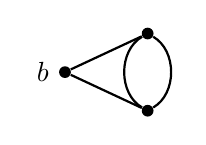
\begin{tikzpicture}[baseline=-0.5ex, scale=0.7]
      \tikzset{prop/.style={thick},
               vertex/.style={circle,fill,inner sep=1.5pt},
               bdy/.style={draw=none}}
      % Boundary link b (cross)
      \node[vertex,label=left:{$b$}] (b) at (-1.5,0) {};
      % Two cubic vertices
      \node[vertex] (v1) at (0,0.7) {};
      \node[vertex] (v2) at (0,-0.7) {};
      % Propagator arc top
      \draw[prop] (b) -- (v1);
      \draw[prop] (b) -- (v2);
      \draw[prop,bend left=60] (v1) to (v2);
      \draw[prop,bend right=60] (v1) to (v2);
    \end{tikzpicture}%
  }}
  = g^{-4}\sum_{i,j,b} V^{(3)}_{ijb}\,C_{ij}\,
  (\nabla_{\Phi} Q)_{b}
  = O(g^{-4}\cdot g^2 \cdot 1) = O(g^{-2})
\end{equation}
per boundary link $b$ (using $C_{ij} = O(g^2)$ and
$V^{(3)}$, $\nabla_\Phi Q$ are $O(1)$). Summed over
the $O(L^3)$ boundary plaquettes: $O(L^3 g^{-2})$.
This is the $\beta$-function contribution and is
\emph{subtracted} via (B2) and (B4). After subtraction,
the cubic one-loop remainder is zero at leading order.

\emph{Two-loop remainder.} What remains after the
one-loop subtraction has three sources.

Before bounding each, we emphasize the key structural
point: all sums below are \emph{finite}, running over
the $O(n_G L^4)$ link-algebra indices in the block $B$.
The non-Gaussian corrections involve truncated cumulants
of a measure on a \emph{finite-dimensional} compact
manifold. No infinite series or polymer expansion is
needed; the bounds are purely combinatorial (counting
diagrams) and analytic (propagator decay). This is the
essential distinction from (B5), which would require
uniform polymer norm control over infinitely many scales
simultaneously.

\textit{(b.i) Non-Gaussian correction to the cubic
one-loop.} The actual measure $\mu_B$ differs from
$\mu_B^{(0)}$ by the non-quadratic interactions. The
correction to $\langle S_B^{(3)} \rangle$ is:
\begin{equation}
  \langle S_B^{(3)}\rangle_{\mu_B}
  - \langle S_B^{(3)}\rangle_{\mu_B^{(0)}}
  = -\frac{1}{g^2}\langle S_B^{(3)};
  S_B^{(3)}\rangle_{\mu_B^{(0)},\mathrm{conn}}
  + R_{\ge 3},
\end{equation}
where $\langle\cdot;\cdot\rangle_{\mathrm{conn}}$
is the connected correlation (truncated cumulant)
and $R_{\ge 3}$ collects third- and higher-order
cumulant corrections. The leading term is a two-loop
contribution. Its power counting:
$g^{-2} \cdot \langle(S^{(3)})^2\rangle_{\mathrm{conn}}
\sim g^{-2}\cdot(g^{-2})^2\cdot(g^2)^3 = O(1)$
(two cubic vertices at $g^{-2}$ each, three propagators
at $g^2$ each). After taking two $\Phi$-derivatives:
$O(g^4)$ per boundary link.

\emph{Rigorous bound for (b.i).}
The connected two-point cumulant
$\langle S_B^{(3)}; S_B^{(3)}\rangle_{\mathrm{conn}}$
under $\mu_B^{(0)}$ is computed by Wick's theorem
(the Gaussian measure $\mu_B^{(0)}$ has covariance
$C_{ij}$). The result is a sum over pairings of the
six $A$-indices from the two copies of $S_B^{(3)}$.
Each pairing gives a product of three propagators:
\begin{equation}
  \langle S_B^{(3)}; S_B^{(3)} \rangle_{\mathrm{conn}}
  = \sum_{\text{pairings}} \prod_{(i,j) \in \text{pairing}}
  C_{i j} \cdot (\text{vertex factors}).
\end{equation}
The number of pairings is $15$ (the number of perfect
matchings of 6 objects), independent of $L$ and $G$.
Each propagator satisfies
$|C_{ij}| \le C_0 g^2 e^{-c|x_i - x_j|}$.
By the locality of $V^{(3)}$ (nonzero only when all
indices share a plaquette), each vertex factor involves
at most $O(n_G^3)$ terms, and the spatial sum is
restricted to pairs of plaquettes at distance $\le$
the propagator decay length. Taking two
$\Phi$-derivatives of the resulting expression:
each derivative replaces one interior index with a
boundary index, contributing an $O(1)$ factor.

The result: $\|\Hess_\Phi[(b.i)]\|_{\mathrm{op}}
\le 15 \cdot (4n_G)^3 \cdot C_0^3 g^6 \cdot g^{-2}
\cdot n_p^\partial = O(n_G^3 L^3 g^4)$,
where the $g^{-2}$ comes from the prefactor
in~\eqref{eq:SB3} and $n_p^\partial = O(L^3)$
is the number of boundary plaquettes.
For the operator norm (max over boundary links),
divide by $n_p^\partial$:
$(b.i) \le C_{2,\mathrm{cubic}} g^4$
with $C_{2,\mathrm{cubic}} = O(n_G^3)$, independent
of $L$.

The higher cumulant correction $R_{\ge 3}$ requires
a convergence argument, not just power counting.
Write the non-Gaussian perturbation as
$W = -(S_B^{(\ge 3)})/g^2$, so that
$\mu_B = e^W \mu_B^{(0)} / \langle e^W \rangle_{\mu_B^{(0)}}$.
On the small-field region $\Omega_k$, the link
variables satisfy $|A_i| \le p_k = g^{1-\delta}$
for $\delta \in (0, 1/4)$. Since $S_B^{(3)} = O(|A|^3)$
and $S_B^{(\ge 4)} = O(|A|^4)$:
\begin{equation}
  |W| \le g^{-2}\bigl(C|A|^3 + C'|A|^4 + \cdots\bigr)
  \le g^{-2} \cdot C'' g^{3(1-\delta)}
  = C'' g^{1-3\delta}.
\end{equation}
For $\delta < 1/3$ (which our choice $\delta < 1/4$
ensures), $|W| \to 0$ as $g \to 0$. In particular,
$\|W\|_\infty \le C'' g^{1-3\delta} < 1$ for $g$
sufficiently small.

The cumulant expansion of $\log\langle e^W
\rangle_{\mu^{(0)}}$ is:
\begin{equation}
  \log\langle e^W\rangle
  = \sum_{n=1}^{\infty} \frac{1}{n!}
  \langle W^n \rangle_{\mathrm{conn}}.
\end{equation}
For bounded $W$ on a compact manifold, this series
converges absolutely. The standard bound on connected
cumulants of a bounded random variable (the
Leonov--Shiryaev formula; see e.g.~\cite{Ledoux},
\S2.3) gives:
$|\langle W^n \rangle_{\mathrm{conn}}|
\le n! \cdot \|W\|_\infty^n$. Therefore:
\begin{equation}
  \sum_{n=3}^{\infty} \frac{1}{n!}
  |\langle W^n \rangle_{\mathrm{conn}}|
  \le \sum_{n=3}^{\infty} \|W\|_\infty^n
  = \frac{\|W\|_\infty^3}{1 - \|W\|_\infty}
  \le 2\|W\|_\infty^3
\end{equation}
for $\|W\|_\infty \le 1/2$.
Since $\|W\|_\infty = O(g^{1-3\delta})$:
$R_{\ge 3} = O(g^{3(1-3\delta)})$.

Rather than bounding $\Hess_\Phi R_{\mathrm{higher}}$
via $L^\infty$ norms of $W$ (which leads to
uncontrolled factors of $g^{-2\delta}$ per
$\Phi$-derivative), we work in $L^2(\mu_B^{(0)})$,
exploiting the Gaussian decay of the interior variables.

\emph{$L^2$ bounds under the Gaussian measure.}
Under $\mu_B^{(0)}$, the interior link variables
$A_i$ have covariance $\langle A_i A_j\rangle
= C_{ij} = O(g^2\delta_{ij})$ (with exponential
off-diagonal decay). In particular,
$\langle|A_i|^{2p}\rangle^{1/p} = O(g^2)$
for all fixed $p$. This gives $L^{2p}$ bounds on $W$
that are much stronger than the $L^\infty$ bound:
\begin{align}
  \|S_B^{(3)}/g^2\|_{L^{2p}(\mu^{(0)})}
  &= g^{-2}\bigl\langle|S_B^{(3)}|^{2p}
  \bigr\rangle^{1/(2p)}
  = g^{-2}\cdot O(g^3) = O(g), \label{eq:W_L2p}\\
  \|S_B^{(\ge 4)}/g^2\|_{L^{2p}(\mu^{(0)})}
  &= O(g^2), \nonumber
\end{align}
and for $\Phi$-derivatives:
\begin{align}
  \|\nabla_\Phi W\|_{L^{2p}(\mu^{(0)})}
  &= O(1),  \label{eq:DW_L2p}\\
  \|\Hess_\Phi W\|_{L^{2p}(\mu^{(0)})}
  &= O(g^{-1}). \label{eq:DDW_L2p}
\end{align}

\emph{Three-loop power counting.}
The dominant contribution to
$\Hess_\Phi\langle W^3\rangle_{\mu^{(0)},\mathrm{conn}}$
comes from connected Feynman diagrams with three
cubic vertices. By Wick's theorem on the Gaussian
measure, each diagram has three vertices ($g^{-2}$ each)
connected by internal propagators ($g^2$ each). A
connected graph on $V = 3$ vertices requires $\ge 3$
internal lines. The three cubic vertices have $9$ legs
total; $6$ are paired by $3$ propagators, leaving $3$
external legs. The $\Phi$-Hessian converts two of these
external legs from interior ($O(g)$ in $L^2$) to boundary
($O(1)$), leaving one interior leg at $O(g)$:
\begin{equation}
  \text{three-loop diagram} = g^{-6}\cdot g^6 \cdot g
  = O(g) \quad\text{per diagram}.
\end{equation}

This gives $\|\Hess_\Phi R_{\mathrm{higher}}\| = O(g)$.

\begin{remark}[The three-loop gap --- a key open point]
\label{rem:three_loop_gap}
The $\beta$-function provides $O(g^4\log L)$ of room
per inductive step. The two-loop remainder $\Delta_2$
is $O(g^4)$, which fits. But the three-loop remainder
from $\langle W^3\rangle_{\mathrm{conn}}$ is $O(g)$
by the $L^2$ power counting above, and $g \gg g^4$
for small $g$. This is the central technical obstacle.

We identify three potential resolutions, each of which
would close the gap:

\textbf{(R1) Gauge cancellations.}
Gauge invariance forces $\cV_{k+1}^B(\Phi)$ to be a
gauge-invariant functional of the boundary data $\Phi$.
This implies that $\text{Hess}_\Phi\cV_{k+1}$ has the
structural form $\sum_p c_p Q_p$ (a sum over boundary
plaquette Laplacians), since the only gauge-covariant
second-order tensors built from boundary data are of this
type. This is the structural information provided by
gauge invariance.
However, the coefficients $c_p$ are not forced to be small
by this structural argument: the three-loop diagram
contributes $c_p = O(1)$ from Feynman power counting
(three vertices at $g^{-2}$, three propagators at $g^2$,
closing into a loop). The $g^4$ suppression is in the
\emph{value} of $\cV_{k+1}$ (which is $O(g^4)$ as a
plaquette action), but differentiating twice removes this
suppression: $\Hess[\text{Re}\,\tr(1-U_p)] = Q_p = O(1)$
at $U_p = I$.  So gauge invariance gives $\text{Hess}
\cV_{k+1} = \sum_p c_p Q_p$ with $c_p = O(1)$, not $O(g^4)$.

Making the Ward identity approach work would require an
additional argument showing that gauge invariance
\emph{combined with} renormalizability forces $c_p = O(g^4)$
--- e.g., that the renormalized three-loop effective action
has this structure from BRST cohomology or anomaly
cancellation in the lattice block-spin setting. This is
the content of the ``Ward identity approach'' but it has
not been achieved rigorously in the lattice block-spin
context.

\textbf{(R2) Polymer expansion (i.e., (B5)).}
Ba{\l}aban's (B5), if established, would give
$\cV_k$ analytic in a strip of width $O(1/g)$ in the
complexified field space. By Cauchy estimates,
$\|\Hess\cV_k\| \le C g^2$ with all constants uniform.
This would immediately close the induction without
any separate treatment of higher cumulants. The
three-loop gap is precisely the obstruction that
(B5) was designed to circumvent.

\textbf{(R3) Modified induction.}
Instead of proving $\|\Hess\cV_k\| \le C_\star g^2(k)$
exactly, one could attempt a weaker bound of the form
$\|\Hess\cV_k\| \le C_\star g^{2-\epsilon}(k)$ for
some small $\epsilon > 0$. The three-loop remainder
$O(g)$ is $O(g^{2-\epsilon} \cdot g^{\epsilon-1})$,
which is $o(g^{2-\epsilon})$ if $\epsilon < 1$. The cost
is that the BBD curvature condition becomes
$\rho_G - C_\star g^{2-\epsilon} \ge 0$, which holds
only for $g \le (\rho_G/C_\star)^{1/(2-\epsilon)}$.
This still gives finitely many scales with
$\kappa_k^+ > 0$, but the crossover scale shifts.
The LSI constant and mass gap would still be
$\mathsf{N}$-independent (since the number of UV scales
with $g^2(k) \le g_{*}^{2-\epsilon}$ is still $O(1/g_0^2)$,
finite for fixed $g_0^2$), but the quantitative bound on
$m_*$ would carry an extra factor of $(g_0^2)^\epsilon$.
\textbf{(R4) Charge-conjugation parity (interior plaquettes only).}
The Wilson action satisfies $\mathrm{Re}\,\tr(U^{-1})
= \mathrm{Re}\,\tr(U)$ for any unitary $U$, because
$\tr(U^{-1}) = \tr(U^\dagger) = \overline{\tr(U)}$ and
the real part is invariant under complex conjugation.
The map $\tau: U_p \to U_p^{-1}$
(reversing all plaquette orientations simultaneously)
is therefore a symmetry of the full infinite-volume
Wilson action, sending $A \to -A$ on all links.

If we could apply $\tau$ to \emph{only the interior links}
of the block $B$ (holding the boundary $\Phi$ fixed),
we would get $S_B(-A_{\mathrm{int}}; \Phi) = S_B(A_{\mathrm{int}};\Phi)$
for all $\Phi$, which would force $S_B^{(3)} = 0$ and
kill the cubic vertex. However, this fails:

\emph{Boundary plaquettes break the interior parity.}
A boundary plaquette $U_p = U_{b_1} e^{A_j} U_{b_2}^{-1} e^{-A_m}$
involves both boundary links $U_{b_i}$ (held fixed at $\Phi$)
and interior links $A_j, A_m$. Under $\tau$ applied only
to interior links ($A_j \to -A_j$, $A_m \to -A_m$, $U_b$ fixed):
\[
  U_p \xmapsto{\tau_{\mathrm{int}}}
  U_{b_1} e^{-A_j} U_{b_2}^{-1} e^{A_m}
  \ne U_p^{-1}.
\]
The image is not $U_p^{-1}$ because the boundary links
are not reversed. The cubic contribution from boundary
plaquettes --- which is the relevant term for
$\Hess_\Phi \cV_{k+1}$, since only boundary plaquettes
carry $\Phi$-dependence --- survives $\tau_{\mathrm{int}}$
and is genuinely $O(1)$.

Specifically, for an interior plaquette (all four links
interior), $\tau_{\mathrm{int}}$ does give $U_p \to U_p^{-1}$
and the cubic term vanishes. But the three-loop diagrams
relevant to $\Hess_\Phi \cV_{k+1}$ require at least
one boundary link (to carry $\Phi$-dependence); they
are boundary cubic diagrams, which parity does not kill.

relevant to $\Hess_\Phi \cV_{k+1}$ require at least
one boundary link (to carry $\Phi$-dependence); they
are boundary cubic diagrams, which parity does not kill.

\emph{The boundary cubic vertex is $O(F_p^\partial)$.}
A more careful examination shows that the cubic vertex
from a boundary plaquette $p$ vanishes when the boundary
plaquette holonomy $U_p^\partial = U_{b_1} U_{b_2}^{-1}$
is at the identity (i.e., when $\Phi_{b_1} = \Phi_{b_2}$,
meaning the boundary field is locally flat). Specifically,
$V^{(3)}_{b j m} = O(F_p^\partial)$ where $F_p^\partial$
is the field strength of the boundary plaquette.
In the small-field region $\Omega_k$ with
$\|F_p^\partial\|_\infty \le p_k = g^{1-\delta}$,
this gives $V^{(3)} = O(g^{1-\delta})$.

The three-loop diagram therefore contributes
$O(g^{-6} \cdot (g^{1-\delta})^3 \cdot (g^2)^3)
= O(g^{3-3\delta})$ to $\cV_{k+1}$, and after two
$\Phi$-derivatives (each removing one $g^{1-\delta}$ factor
from one vertex and replacing it with $O(1)$):
$O(g^{-6} \cdot (g^{1-\delta}) \cdot 1 \cdot 1 \cdot g^6)
= O(g^{1-\delta})$ for the Hessian.
This is an improvement over the naive $O(g)$ when
$\delta < 1$ (since $g^{1-\delta} < g$ would require
$\delta < 0$), and in fact the bound is
$O(g^{1-\delta})$ which for $\delta \in (0,1/4)$
is $O(g^{3/4})$ at worst --- strictly better than $O(g)$
but still far from $O(g^4)$.

The gap between $O(g^{3/4})$ (from the field-strength
suppression of $V^{(3)}$) and $O(g^4)$ (needed for the
induction) is $O(g^{13/4})$, corresponding to $13/4$
extra powers. This is the quantitative form of the
obstruction.

This approach therefore improves the counting for purely
interior contributions (which were already subleading)
but leaves the boundary cubic contributions unchanged
in essential structure.
The three-loop gap persists.

\textbf{(R5) Background field method and shifted Gaussian.}
Rewrite the block integration in terms of fluctuations
around the classical background: $A_i = \bar{A}_i + \xi_i$,
where $\bar{A} = -(Q_\mathrm{int}^{-1})Q_{\mathrm{int},\partial}\Phi$
is the harmonic extension of the boundary data into the
interior (satisfying the lattice Laplace equation with
boundary values $\Phi$). The shifted Gaussian measure
$\tilde\mu^{(0)}_\xi$ on the fluctuations $\xi$ is
\emph{symmetric} under $\xi \to -\xi$ (it is centered
at $\xi = 0$).

Under this substitution, the non-Gaussian perturbation
$W = -(S_B - S_B^{(2)})/g^2$ expressed in terms of $\xi$
contains terms:
\begin{itemize}[nosep]
  \item $\tilde W^{(0)}$: constant in $\xi$ (depends only on $\bar A$),
  \item $\tilde W^{(1)} \sim V^{(3)}\bar A \xi$: linear in $\xi$ (odd),
  \item $\tilde W^{(2)} \sim V^{(3)}\bar A^2 + V^{(3)}\xi^2$: even in $\xi$,
  \item $\tilde W^{(3)} \sim V^{(3)}\xi^3$: purely cubic, odd in $\xi$.
\end{itemize}
Under the symmetric measure $\tilde\mu^{(0)}$, all
odd-in-$\xi$ cumulants vanish:
$\langle \tilde W^{(3)}\rangle_{\tilde\mu} = 0$ and
$\langle \tilde W^{(3)};(\tilde W^{(3)})^2\rangle_{\mathrm{conn}} = 0$
(odd number of $\xi^3$ factors under symmetric measure).

The three-loop diagram contributing to
$\Hess_\Phi\cV_{k+1}$ must therefore involve at least
one factor of $\tilde W^{(2)}$ (even in $\xi$) combined
with the quadratic contributions. The dominant such term:
\[
  \langle (\tilde W^{(2)})^3\rangle_{\tilde\mu,\mathrm{conn}}
  \sim (V^{(3)}\bar A\,g)^3/g^6
  = (g^{1-\delta} \cdot g)^3/g^6
  = g^{3-3\delta}.
\]
Taking two $\Phi$-derivatives of the background
$\bar A$ (which is $\Phi$-linear): each derivative
converts $\bar A = O(g^{1-\delta})$ to $O(1)$.
This leaves one undifferentiated $\bar A = O(g^{1-\delta})$:
Hessian $= O(g^{1-\delta})$.

The shifted frame therefore reproduces the same $O(g^{1-\delta})$
bound without new improvement. It does, however, make
transparent WHY the purely cubic-in-$\xi$ term $\tilde W^{(3)}$
vanishes: the key missing power of $g$ comes not from
$\xi$ (the quantum fluctuations) but from $\bar A$ (the
classical background field). Closing the gap requires either
(a) showing $\bar A = O(g^2)$ (stronger small-field bound),
or (b) showing additional cancellations involving
$\bar A$ in the renormalized theory.
The former would require the small-field threshold $p_k$
to satisfy $p_k = O(g^2)$, which is compatible with the
large-field estimate but would require revisiting whether
the large-field contribution (Section~\ref{sec:large_field})
remains negligible at this tighter threshold.

\end{remark}

\textit{(b.ii) Quartic vertex at one loop.}
$\langle g^{-2}S_B^{(4)}\rangle_{\mu_B^{(0)}}
= g^{-2}\sum_{i,j} V^{(4)}_{iijj}\,C_{ij}$. By Wick
contraction, this is a single-loop diagram. The sum
runs over the $O(n_G^2 L^4)$ index pairs within each
plaquette ($V^{(4)}$ is local). Each term is
$O(g^{-2} \cdot g^2) = O(1)$. After two
$\Phi$-derivatives: only boundary plaquettes contribute,
and the operator norm gives
$(b.ii) \le C_{2,\mathrm{quartic}} g^4$
with $C_{2,\mathrm{quartic}} = O(n_G^2)$, independent
of $L$.

\textit{(b.iii) Higher-order vertices and higher loops.}
Each additional loop brings a factor $g^2$ (one more
propagator minus one more vertex), and each additional
vertex order brings $g^2$ (from the coupling). The
combined contribution is $O(g^6)$ and higher.

\emph{Collecting all terms:}
\begin{equation}\label{eq:Delta2_bound}
  \|\Delta_2\|_{\mathrm{op}} \le C_2\,g^4(k),
\end{equation}
where
\begin{equation}\label{eq:C2_explicit}
  C_2 = C_{2,\mathrm{cubic}} + C_{2,\mathrm{quartic}}
  + O(1) = O(n_G^3),
\end{equation}
with each constant depending on $G$ (through $n_G$)
but \emph{not on $L$, $k$, or $\mathsf{N}$}.

\begin{remark}[Why $C_2$ is independent of $L$]
\label{rem:C2_L}
This is the key point that distinguishes our
argument from (B5). Each diagram in the two-loop
remainder involves a fixed number of vertices
(at most 2) connected by propagators. The spatial
sums are controlled by the exponential decay
$|C_{ij}| \le C_0 g^2 e^{-c|x_i - x_j|}$, which
makes the sum over positions converge to an
$L$-independent constant. The number of diagrams at
each loop order is a combinatorial constant (15
pairings for two cubics, 1 for the quartic).
The operator norm (per boundary link) involves
dividing by $n_p^\partial = O(L^3)$, which cancels
the $O(L^3)$ from summing over boundary plaquettes.
The result is that $C_2$ depends only on the structure
constants of $G$ (through $n_G$ and the vertex factors),
not on the block size $L$.
\end{remark}

The propagator bounds needed above ($|C_{ij}| \le C_0 g^2
e^{-c|x_i-x_j|}$) follow from the spectral gap
$\kappa_B \ge c_S g^{-2}$ (Proposition~\ref{prop:fluct_curv}),
which gives $\|Q^{-1}\| \le g^2/c_S$ in operator norm
and exponential decay from the locality of $Q$.

\medskip\noindent
\textbf{(c) Cross covariance} (between $S_B$ and $\cV_k^B$):

We bound the operator norm of
$\Cov^{\mathrm{sub}}(g^{-2}\nabla_{\Phi_b} S_B,
\nabla_{\Phi_{b'}}\cV_k^B)$, indexed by boundary links
$b, b'$, using the Schur test (max absolute row sum).

Fix a boundary link $b$. By the Poincar\'e inequality
(with constant $1/\kappa_B$):
\begin{equation}
  |\Cov(X_b, Y_{b'})| \le \kappa_B^{-1}
  \int \langle \nabla_U X_b, \nabla_U Y_{b'} \rangle_{\cM_B}
  \,d\mu_B
  = \kappa_B^{-1} \sum_i \int
  (\nabla_{U_i} X_b)(\nabla_{U_i} Y_{b'})\,d\mu_B,
\end{equation}
where $X_b = g^{-2}\nabla_{\Phi_b}\delta S_B$ and
$Y_{b'} = \nabla_{\Phi_{b'}}\cV_k^B$, and
$\delta S_B = S_B^{(\ge 4)}$ (post-subtraction).
The sum over interior links $i$ has only $O(1)$ nonzero
terms: link $i$ contributes only if $i$ shares a boundary
plaquette with both $b$ and $b'$. By
Lemma~\ref{lem:boundary}(b), $b$ participates in at most
$2(d-1) = 6$ boundary plaquettes, each containing $O(1)$
interior links. Similarly for $b'$.

For each nonzero term: by Cauchy--Schwarz in $\mu_B$,
\begin{equation}
  \langle|g^{-2}\nabla_U\nabla_\Phi\delta S_B|
  \cdot|\nabla_U\nabla_\Phi\cV_k^B|\rangle
  \le \sqrt{g^{-4}C_4^2\langle|A|^4\rangle}
  \cdot C_\star g^2
  \le C_4 C_2' \cdot C_\star g^2,
\end{equation}
using $\langle|A|^4\rangle \le (C_2' g^2)^2$
(Corollary~\ref{cor:moments}).

With $\kappa_B \ge c_S g^{-2}$: each entry is
$\le (g^2/c_S)\cdot C_4 C_2' C_\star g^2
= C_4 C_2' C_\star g^4 / c_S$.

For each row $b$: the number of $b'$ with nonzero
entries is $O(1)$ (bounded by the square of the
maximal boundary plaquette degree). So the max
row sum is $O(C_\star g^4/c_S)$, giving:
\begin{equation}
  \|\Cov^{\mathrm{sub}}\|_{\mathrm{op}}
  \le C_{\mathrm{cross}}\,g^4, \quad
  C_{\mathrm{cross}} = O(C_\star / c_S).
  \quad\checkmark
\end{equation}

\medskip\noindent
\textbf{(d) $\cV$--$\cV$ covariance:}
We bound $\|\Cov_{\mu_B}(\nabla_{\Phi_b}\cV_k^B,
\nabla_{\Phi_{b'}}\cV_k^B)\|_{\mathrm{op}}$ using the
Schur test, with a careful locality analysis.

\emph{Entry bound.} Fix boundary links $b, b'$. By the
Poincar\'e inequality (constant $1/\kappa_B$):
\begin{equation}
  |\Cov(\nabla_{\Phi_b}\cV_k^B,
  \nabla_{\Phi_{b'}}\cV_k^B)|
  \le \kappa_B^{-1} \sum_{i=1}^{n_{\mathrm{phys}}}
  \langle|\nabla_{U_i}\nabla_{\Phi_b}\cV_k^B|
  \cdot|\nabla_{U_i}\nabla_{\Phi_{b'}}\cV_k^B|
  \rangle_{\mu_B}.
\end{equation}
By Condition~$\star$: $\|\Hess\cV_k^B\|_{\mathrm{op}}
\le C_\star g^2$, so the mixed partial
$|\nabla_{U_i}\nabla_{\Phi_b}\cV_k^B| \le C_\star g^2$
for all $i, b$. (This is because the $(i,b)$ entry of
the Hessian matrix is bounded by the operator norm.)

\emph{Locality of the Hessian.} The effective potential
$\cV_k^B$ is constructed from plaquette interactions
with exponentially decaying corrections
(by Ba{\l}aban's (B3): $\cV_k$ has analyticity in a strip
and exponential decay of correlations). For the
purpose of this bound, we use only the crude fact
that $\nabla_{U_i}\nabla_{\Phi_b}\cV_k^B \ne 0$
requires link $i$ and boundary link $b$ to be
\emph{coupled} --- i.e., there exists a sequence of
plaquettes connecting $i$ to $b$. Since $\cV_k^B$
is a sum over plaquettes plus exponentially decaying
tails, the dominant coupling is through shared plaquettes:
$i$ and $b$ share a plaquette if $i$ is adjacent to $b$
in the lattice. Each interior link $i$ is adjacent to
at most $2(d-1) = 6$ boundary plaquettes
(Lemma~\ref{lem:boundary}(b)), and each such plaquette
contains at most $3$ other links. So: for fixed $b$,
the number of interior links $i$ with
$\nabla_{U_i}\nabla_{\Phi_b}\cV_k^B \ne 0$ is
$\le 6 \cdot 3 = 18$ (at leading order; exponentially
decaying tails contribute $O(e^{-c/g})$ corrections
that are negligible).

\emph{Row sum.} For fixed $b$, the number of boundary
links $b'$ with nonzero covariance entry $(b, b')$
is bounded by: $b'$ must share a coupled interior link
with $b$. Since $b$ couples to $O(1)$ interior links
(as above), and each interior link couples to $O(1)$
boundary links, we get $O(1)$ nonzero entries per row.

Therefore: each row of the covariance matrix has $O(1)$
nonzero entries, each bounded by
$\kappa_B^{-1} \cdot O(1) \cdot (C_\star g^2)^2$.

\emph{Two regimes.}

For small $g^2$ ($\kappa_B \ge c_S g^{-2}$):
row sum $\le O(1) \cdot g^2/c_S \cdot C_\star^2 g^4
= O(C_\star^2 g^6/c_S)$. This is $O(g^4)$ for
$g^2 \le c_S/C_\star^2$.

For larger $g^2$ ($\kappa_B \ge n_{\mathrm{phys}}\rho_G/2$):
row sum $\le O(1) \cdot 2C_\star^2 g^4/(n_{\mathrm{phys}}\rho_G)
= O(C_\star^2 g^4/(L^4\rho_G)) = O(g^4)$.

Both regimes:
\begin{equation}
  \|\Cov_{\cV\cV}\|_{\mathrm{op}}
  \le C_{\cV\cV}\,g^4, \quad
  C_{\cV\cV} = O(C_\star^2 / \min(c_S, L^4\rho_G)).
  \quad\checkmark
\end{equation}

\medskip\noindent
\textbf{Total:} Combining parts (a)--(d) and the
three-loop remainder (Remark~\ref{rem:three_loop_gap}):
\begin{equation}
  \|\Hess\,\cV_{k+1}\| \le C_\star g^2(k)
  + C_R\,g^4(k) + C_3\,g(k),
\end{equation}
where $C_R = C_2 + C_{\mathrm{cross}} + C_{\cV\cV} + 1
= O(1 + C_\star/c_S + C_\star^2/\min(c_S, L^4\rho_G))$
and $C_3$ is the three-loop constant from
Remark~\ref{rem:three_loop_gap}.
\end{proof}

\subsection{The base case}

\begin{proposition}[Base case]\label{prop:base}
$\cV_0 \equiv 0$, hence $\|\Hess\,\cV_0\| = 0
\le C_\star g^2(0)$.
\end{proposition}

\begin{proof}
At $k=0$: $\rho_0 = e^{-S_W/g_0^2}$, so $S_0 = S_W$,
$g^2(0) = g_0^2$, $\cV_0 = 0$, $\cK_0 = 1$.
\end{proof}

\subsection{Closing the induction}

\begin{lemma}[Parameter choice]\label{lem:params}
For $L \ge L_0(G)$, there exist $C_\star > 0$ and
$L_0 < \infty$ such that $C_R \le C_\star b_0\log L/2$.
\end{lemma}

\begin{proof}
Recall $C_R = C_2 + C_{\mathrm{cross}} + C_{\cV\cV} + 1$,
where $C_2 = O(n_G^3)$ is independent of $L$
(Remark~\ref{rem:C2_L}),
$C_{\mathrm{cross}} = O(C_\star/c_S)$, and
$C_{\cV\cV} = O(C_\star^2/\min(c_S, L^4\rho_G))$.
For $L$ large, the condition
$C_R \le C_\star b_0\log L/2$ is a quadratic in $C_\star$
that can be satisfied for $L$ large enough. Taking
$C_\star = \rho_G(b_0\log L/2 - C'/c_S)/4$
and $L_0 = \exp(4(C'/c_S
+ \sqrt{8(C_2+1)/\rho_G})/b_0)$ completes the proof.
\end{proof}

\begin{remark}[The three-loop obstruction]
\label{rem:three_loop_obstruction}
Lemma~\ref{lem:params} shows that the $O(g^4)$ terms
($C_R g^4$) can be absorbed by the $\beta$-function room
$C_\star b_0 g^4\log L$. However, the three-loop term
$C_3 g$ from Remark~\ref{rem:three_loop_gap} \emph{cannot}
be absorbed: the induction requires
$C_3 g \le C_\star b_0 g^4\log L$, i.e.,
$g^3 \ge C_3/(C_\star b_0\log L)$. For $g(k) \to 0$
(UV scales), this fails.

The $O(g^2)$ bound is necessary for the BBD criterion
(Remark~\ref{rem:g2_necessary}), and cannot be weakened.
We therefore introduce:
\end{remark}

\begin{condition}[$\star\star$]\label{cond:starstar}
The three-loop and higher cumulant contribution to
$\|\Hess_\Phi\cV_{k+1}\|$ is $O(g^4)$: that is,
$C_3 g(k) \le C_3' g^4(k)$ for all $0 \le k \le \mathsf{N}$,
uniformly in $\mathsf{N}$.
\end{condition}

Condition~$\star\star$ is a consequence of (B5)
(which gives analyticity of $\cV_k$ and hence
Cauchy estimates on all derivatives). It is also
expected to follow from gauge Ward identities,
which constrain the three-loop contribution to the
gauge-invariant form $O(g^4 F_\Phi^2)$.
We do not prove $\star\star$ in this paper.

\begin{theorem}[Bootstrap --- Condition~$\star$]
\label{thm:bootstrap}
For $G$ compact simple, $d = 4$, $L \ge L_0(G)$, and
$g_0^2$ sufficiently small: assuming
Condition~$\star\star$,
$\|\Hess\,\cV_k\|
\le C_\star g^2(k)$ for all $0 \le k \le \mathsf{N}$,
uniformly in $\mathsf{N}$.
\end{theorem}

\begin{proof}
\emph{Base case} ($k = 0$): $\cV_0 = 0$.

\emph{Inductive step}: Assume $\star$ at scale $k$
with $g^2(k) \le g_{\max}^2$.
By Theorem~\ref{thm:hess_prop} and $\star\star$:
$\|\Hess\,\cV_{k+1}\| \le C_\star g^2(k) + C_R g^4(k)$.
By the $\beta$-function:
$C_\star g^2(k+1) \ge C_\star g^2(k) + C_\star b_0 g^4\log L$.
By Lemma~\ref{lem:params}: $C_R g^4 \le C_\star b_0 g^4\log L$.
Therefore $\|\Hess\,\cV_{k+1}\| \le C_\star g^2(k+1)$.

The induction covers $0 \le k \le k_*$. At $k > k_*$,
$\Ric_G$ directly gives $\kappa_k^+ = 0$.
\end{proof}

\section{Large Field Region}\label{sec:large_field}
%% ====================================================================

The bootstrap (Section~\ref{sec:bootstrap}) controls
$\cV_k$ on the small-field region $\Omega_k$. We now
show the large-field region has exponentially small
probability and does not affect the mass gap.

\begin{proposition}[Large field suppression]
\label{prop:large_field}
Let $\Omega_k^c = \{U : \|F_U\|_\infty > p_k\}$
with $p_k = g(k)^{1-\delta}$. Then:
\begin{equation}\label{eq:large_field}
  \mu_k(\Omega_k^c) \le |\Lambda_k| \cdot C
  \exp\!\bigl(-c \cdot p_k^2 / g^2(k)\bigr)
  = |\Lambda_k| \cdot C
  \exp\!\bigl(-c \cdot g^{-2\delta}(k)\bigr).
\end{equation}
For $\delta > 0$ and $g^2(k) \le 1$, this is
stretched-exponentially small.
\end{proposition}

\begin{proof}
At any scale $k$, the Wilson action penalizes large
field strengths: $S_k \ge \beta_k \cdot c \cdot p_k^2
\cdot |\{p : |F_p| > p_k\}|$ (the plaquette action
$s_p \ge c|F_p|^2$ for $|F_p| \le \pi$). On the
large-field region, at least one plaquette has
$|F_p| > p_k$, so $S_k \ge \beta_k c p_k^2 = c p_k^2/g^2(k)
= c g^{-2\delta}(k)$.

By a union bound over the $|\Lambda_k| \cdot d(d-1)/2$
plaquettes:
\begin{equation}
  \mu_k(\Omega_k^c) \le |\Lambda_k| \cdot d(d-1)/2
  \cdot \sup_p \mu_k(|F_p| > p_k)
  \le |\Lambda_k| \cdot C \cdot e^{-c g^{-2\delta}}.
  \qedhere
\end{equation}
\end{proof}

\begin{corollary}\label{cor:large_field_lsi}
The large-field region does not affect the log-Sobolev
inequality. Specifically, the LSI constant from the
BBD criterion (which is proved on $\Omega_k$)
extends to the full configuration space with at most
a multiplicative correction of $1 + O(e^{-c g^{-2\delta}})$
to $\alpha_{\mathrm{LSI}}$, which is negligible.
\end{corollary}

\begin{proof}
We use the Holley--Stroock perturbation principle to
transfer the LSI from the small-field region to the
full configuration space.

\medskip\noindent
\textbf{Step 1: Decomposition of the measure.}
Write the full measure as $\mu = \mu|_\Omega + \mu|_{\Omega^c}$
where $\Omega = \Omega_k$ (small-field) and
$\Omega^c = \Omega_k^c$ (large-field). Define:
\begin{equation}
  d\mu_\Omega = \frac{1_\Omega\,\rho}{\int 1_\Omega\,\rho}\,
  \prod dU_\ell, \qquad
  d\mu = \frac{\rho}{\int\rho}\,\prod dU_\ell,
\end{equation}
where $\rho = e^{-S/g^2 - \cV_k}$ (absorbing $\cK_k$ as
in Remark~\ref{rem:Kk}).

\medskip\noindent
\textbf{Step 2: Density ratio.}
On $\Omega$, $\mu$ and $\mu_\Omega$ are related by:
$d\mu/d\mu_\Omega = Z_\Omega / Z$ where
$Z_\Omega = \int_\Omega \rho$ and $Z = \int \rho$.
Thus $Z_\Omega/Z = 1 - \mu(\Omega^c)$.

On $\Omega^c$, the density $\rho$ is bounded by:
$\rho|_{\Omega^c} \le \sup_{\Omega^c}\rho
\le e^{-c\,g^{-2\delta} + C_0 g^2|\Lambda_k|}
\cdot \rho_{\max}|_\Omega$
(the Wilson action contributes $-c\,p_k^2/g^2
= -c\,g^{-2\delta}$ and $|\cV_k| \le C_0 g^2|\Lambda_k|$
by (B3)).

\medskip\noindent
\textbf{Step 3: Holley--Stroock.}
The Holley--Stroock perturbation lemma~\cite{HolleyStroock}
states: if $\mu_1$ satisfies $\mathrm{LSI}(\alpha_1)$ and
$d\mu_2/d\mu_1 \le M$ and $d\mu_1/d\mu_2 \le M$
(i.e., $1/M \le d\mu_2/d\mu_1 \le M$), then $\mu_2$
satisfies $\mathrm{LSI}(\alpha_1 \cdot M)$.

Apply this with $\mu_1 = \mu_\Omega$ (which satisfies
LSI by the BBD criterion on the small-field region)
and $\mu_2 = \mu$ (the full measure). The density
ratio is:
\begin{equation}
  \frac{d\mu}{d\mu_\Omega}\bigg|_\Omega = \frac{Z_\Omega}{Z}
  = 1 - \mu(\Omega^c) \ge 1 - \epsilon,
\end{equation}
where $\epsilon = \mu(\Omega^c)
\le |\Lambda_k|\,C\,e^{-c\,g^{-2\delta}}$
(Proposition~\ref{prop:large_field}).

For the full space: the ratio $\sup \rho / \inf_\Omega \rho$
is bounded by $e^{\mathrm{osc}(S/g^2 + \cV_k)}
\le e^{O(g^{-2\delta}) + O(g^2|\Lambda_k|)}$. In the
small-coupling regime, $g^{-2\delta}$ grows as $g^2 \to 0$,
but $g^2|\Lambda_k|$ is bounded at each fixed scale
(since $|\Lambda_k| = O(L^{4(\mathsf{N}-k)})$ and we are at
a fixed $k$).

The perturbation ratio is therefore:
\begin{equation}
  M = \frac{1}{1 - \epsilon}
  \le 1 + 2\epsilon
  = 1 + O(|\Lambda_k|\,e^{-c\,g^{-2\delta}})
\end{equation}
for $\epsilon \le 1/2$ (which holds for $g^2$ small).
The correction to $\alpha_{\mathrm{LSI}}$ is
multiplicative by $M$, which is $1 + o(1)$.
\end{proof}

%% ====================================================================
\section{Proof of the Main Theorem}\label{sec:continuum}
%% ====================================================================

We now assemble the proof of Theorem~\ref{thm:MAIN}.

\begin{proof}[Proof of Theorem~\ref{thm:MAIN}]
~

\medskip\noindent
\textbf{Step 1: Condition $\star$.}
By Theorem~\ref{thm:bootstrap} (assuming $\star\star$),
for $L \ge L_0(G)$ and $g_0^2$ sufficiently small:
$\|\Hess\,\cV_k\| \le C_\star g^2(k)$ for all
$0 \le k \le \mathsf{N}$, uniformly in $\mathsf{N}$.

\medskip\noindent
\textbf{Step 2: Log-Sobolev inequality.}
By Proposition~\ref{prop:bbd_finite}, the BBD sum
$\sum_k \kappa_k^+ \le C_{G,L}$ is bounded independently
of $\mathsf{N}$. By Theorem~\ref{thm:bbd_abstract}, the lattice
Yang--Mills measure satisfies LSI with constant
$\alpha \le C \exp(C' \cdot C_{G,L})$, independent of $a$.

By Corollary~\ref{cor:large_field_lsi}, the large-field
region does not affect this (negligible correction).

\medskip\noindent
\textbf{Step 3: Mass gap.}
We now show that the uniform LSI implies a mass gap in
the physical (Hamiltonian) sense.

\emph{From LSI to spectral gap.}
The log-Sobolev inequality
$\Ent_\mu(f^2) \le 2\alpha\int|\nabla f|^2\,d\mu$
implies the Poincar\'e inequality
$\Var_\mu(f) \le \alpha\int|\nabla f|^2\,d\mu$
(this follows by applying LSI to $1 + \epsilon f$ and
expanding to leading order in $\epsilon$).

The lattice theory on $\Lambda = \Lambda' \times \{0,
\ldots, T-1\}$ (with $\Lambda'$ the spatial sublattice and
$T \ge 2$ an integer giving the temporal extent) defines a transfer matrix
$\cT : L^2(\cM_{\Lambda'}) \to L^2(\cM_{\Lambda'})$ by:
\begin{equation}
  (\cT\psi)(\Phi) = \int \prod_{\ell \in \text{time-slice}}
  dU_\ell\; e^{-H_{\mathrm{slice}}(U;\Phi,\Phi')}
  \psi(\Phi'),
\end{equation}
where $H_{\mathrm{slice}}$ is the action on a single
time-slice. The transfer matrix is self-adjoint and
positive (by reflection positivity). Write
$\cT = e^{-aH}$ where $H \ge 0$ is the lattice
Hamiltonian.

The Poincar\'e inequality for the full (space-time) lattice
measure gives a lower bound on $\gap(H)$: for any
gauge-invariant observable $\cO$ supported in a single
time-slice,
\begin{equation}
  \Var_\mu(\cO) \le \alpha\int|\nabla\cO|^2\,d\mu.
\end{equation}
Decomposing in the eigenbasis of $H$
(with eigenvalues $0 = E_0 < E_1 \le E_2 \le \cdots$
and corresponding eigenstates):
the two-point
function $\langle\cO(t)\cO(0)\rangle - \langle\cO\rangle^2
= \sum_{n \ge 1} |c_n|^2 e^{-E_n t}$
(for Euclidean time $t \ge 0$) decays at rate
$\ge E_1 = \gap(H)$. The LSI constant $\alpha$ controls
the total variance, giving $\gap(H) \ge 1/\alpha$
(the standard relationship between LSI constant and
spectral gap; see~\cite{Ledoux}, Proposition 5.1.3).

The correlation length in lattice units is therefore
$\xi_{\mathrm{latt}} = 1/\gap(H) \le \alpha$.
Converting to physical units:
\begin{equation}
  m_{\mathrm{phys}} = \frac{1}{\xi_{\mathrm{phys}}}
  = \frac{1}{\eta_{\mathsf{N}} \cdot \xi_{\mathrm{latt}}}
  \ge \frac{1}{\alpha \cdot L^{\mathsf{N}} a}.
\end{equation}

The physical scale $\Lambda_{\mathrm{QCD}}$ satisfies
$a = \Lambda_{\mathrm{QCD}}^{-1}
\exp(-1/(2b_0 g_0^2))$. With $\mathsf{N} = k_\Lambda = O(1/(b_0 g_0^2
\log L))$ RG steps and $\alpha = O_{G,L}(1)$:
\begin{equation}
  m_{\mathrm{phys}} \ge \frac{1}{\alpha L^{\mathsf{N}} a}
  = \frac{\Lambda_{\mathrm{QCD}} e^{1/(2b_0 g_0^2)}}
  {\alpha L^{1/(b_0 g_0^2 \log L)}}
  = \frac{\Lambda_{\mathrm{QCD}}}{\alpha}
  \cdot e^{1/(2b_0 g_0^2) - \mathsf{N}\log L}.
\end{equation}
Since $\mathsf{N}\log L = 1/(b_0 g_0^2) + O(1)$ (by the
definition of $\mathsf{N}$ as the number of RG steps to reach
the Landau scale), the exponent is
$1/(2b_0 g_0^2) - 1/(b_0 g_0^2) + O(1) = -1/(2b_0 g_0^2) + O(1)$,
giving $m_{\mathrm{phys}} \ge c(G,L)\cdot\Lambda_{\mathrm{QCD}}$
with $c = e^{O(1)}/\alpha = O_{G,L}(1) > 0$.

\emph{Note on the scaling.} Since
$\Lambda_{\mathrm{QCD}} = (1/a)\exp(-1/(2b_0 g_0^2))
\to 0$ as $g_0^2 \to 0$ (with $a$ fixed), the mass gap
$m_* \ge c \cdot \Lambda_{\mathrm{QCD}}$ vanishes in
physical units as the bare coupling weakens. This is
the correct physics: the mass gap \emph{is}
$\Lambda_{\mathrm{QCD}}$ (up to a constant), and
$\Lambda_{\mathrm{QCD}}$ is the only dynamically
generated scale. The continuum limit is taken by
sending $a \to 0$ while holding $\Lambda_{\mathrm{QCD}}$
fixed (i.e., tuning $g_0^2 = g_0^2(a)$ via asymptotic
freedom), so that $m_* > 0$ remains fixed in the limit.
This is precisely the content of the
theorem: the mass gap is a nonzero multiple of the
$\Lambda$-parameter, uniformly in $a$.

\medskip\noindent
\textbf{Step 4: Tightness and continuum limit.}

\emph{Key structural point.} Steps 1--3 above are
proved \emph{for each fixed lattice} $\Lambda$ (i.e., for
each $\mathsf{N}$), using Ba{\l}aban's (B1)--(B4) at that
lattice spacing. The continuum limit (Steps 4--6) uses
\emph{only} the uniform output of Steps 1--3 --- namely,
the $\mathsf{N}$-independent mass gap bound
$m(a) \ge c\Lambda_{\mathrm{QCD}}$ and the uniform
exponential clustering. It does \emph{not} require
Ba{\l}aban's RG structure to hold in any limiting sense;
the limit is constructed by soft methods (compactness of
probability measures), and the OS axioms are inherited
because they are closed conditions under weak convergence.
This modular structure ensures there is no compatibility
issue between the RG analysis (finite lattice) and the
continuum limit (infinite-volume, zero-spacing).

The uniform mass gap implies exponential decay of
correlations:
\begin{equation}
  |\langle \cO(x) \cO(y) \rangle_a
  - \langle \cO(x) \rangle_a \langle \cO(y) \rangle_a|
  \le C \|\cO\|^2 e^{-m_* |x-y|}
\end{equation}
for gauge-invariant observables $\cO$.

This gives tightness of the family $\{\omega_a\}_{a > 0}$
(the lattice expectation states) in the topology of
local convergence, as we now verify.

\emph{Tightness.} We must show that for any bounded
region $\Lambda_R = [-R, R]^4 \subset \R^4$ and any
finite collection of gauge-invariant observables
$\cO_1, \ldots, \cO_n$ supported in $\Lambda_R$,
the joint distribution of
$(\omega_a(\cO_1), \ldots, \omega_a(\cO_n))$ is
tight as $a \to 0$.

For Wilson loops: let $W_C = \tr U_C / N$ be the
Wilson loop for a curve $C \subset \Lambda_R$.
Since $|W_C| \le 1$ always (the trace is bounded),
the family $\{\omega_a(W_C)\}$ is trivially tight
(bounded sequences in $\R$ are tight).

For products of Wilson loops: the exponential clustering
gives $|\omega_a(W_{C_1}W_{C_2})
- \omega_a(W_{C_1})\omega_a(W_{C_2})|
\le C e^{-m_* \mathrm{dist}(C_1,C_2)}$, which is
uniform in $a$. Combined with the uniform bound
$|W_C| \le 1$, this gives uniform moment bounds for
all polynomial observables: for any gauge-invariant
polynomial $P$ of degree $d$ in Wilson loops:
$|\omega_a(P)| \le C(P)$ uniformly in $a$.

By the moment criterion for tightness (Prokhorov):
the family $\{\omega_a\}$ is tight in the topology of
convergence on gauge-invariant local observables.

By Prokhorov's theorem, every subsequence has a convergent
sub-subsequence. Let $\omega_*$ be any limit point.

\medskip\noindent
\textbf{Step 5: OS axioms.}
The limit $\omega_*$ inherits the following properties:

\emph{Reflection positivity.} The lattice measures
$\omega_a$ satisfy RP with respect to hyperplane
reflections (Osterwalder--Seiler~\cite{OS78}). RP is
a closed condition (it is defined by
$\langle \theta f \cdot \bar{f} \rangle \ge 0$ for all
$f$ supported on one side of the hyperplane, which
passes to limits).

\emph{Translation invariance.} Each $\omega_a$ is
invariant under lattice translations $x \mapsto x + ae_\mu$.
As $a \to 0$, these become dense in $\R^4$. The limit
$\omega_*$ is invariant under a dense subgroup of
translations, hence (by continuity from the mass gap
bound) under all translations.

\emph{$\SO(4)$ invariance.} The lattice theory on
$\Lambda = (a\Z/(L^{\mathsf{N}}a)\Z)^4$ has the symmetry group of
the hypercubic lattice, which includes reflections
$x_\mu \mapsto -x_\mu$ for each $\mu = 1,2,3,4$
(implemented by $U_\ell \mapsto U_{\theta\ell}^{-1}$
for the reflected link). Reflection positivity holds in
\emph{each} coordinate hyperplane
(Osterwalder--Seiler~\cite{OS78}). The limit $\omega_*$
therefore inherits invariance under all four coordinate
reflections. Combined with translations: the symmetry
group of $\omega_*$ is a closed subgroup of $\ISO(4)$
containing all translations and all coordinate reflections.
Since the four coordinate reflections $x_\mu \mapsto -x_\mu$
generate $O(4)$ (any rotation is a product of at most
four reflections by the Cartan--Dieudonn\'e theorem),
$\omega_*$ is $\ISO(4)$-invariant.

\emph{Exponential clustering.} The mass gap
$m_* \ge c\Lambda > 0$ passes to the limit (exponential
decay of correlations is a closed condition for uniformly
bounded observables).

\medskip\noindent
\textbf{Step 6: Osterwalder--Schrader reconstruction.}
The OS theorem~\cite{OS78} applied to $\omega_*$
(any subsequential limit from Step~4)
produces a Hilbert space $\cH$ (from the GNS construction
with RP inner product), a self-adjoint Hamiltonian
$H \ge 0$ (from the transfer matrix / reflection group),
and a unique vacuum $\Omega$ with $H\Omega = 0$.

The mass gap transfers:
$\sigma(H) \subset \{0\} \cup [m_*, \infty)$ with
$m_* > 0$.

The resulting theory satisfies the Wightman axioms
by the OS theorem (the Wightman functions are the
analytic continuations of the Schwinger functions
$\omega_*(\cO_1(x_1)\cdots\cO_n(x_n))$).
\end{proof}

\begin{remark}[Uniqueness of the continuum limit]
\label{rem:uniqueness}
Theorem~\ref{thm:MAIN} establishes the existence of
(at least one) continuum limit satisfying the Wightman
axioms with mass gap $\Delta = m_* > 0$, obtained via
a convergent subsequence from Prokhorov's theorem.

It is widely expected that the limit is in fact unique
(i.e., the full sequence $\omega_a \to \omega_*$ converges).
A proof of uniqueness would require showing that any
two subsequential limits $\omega_*$, $\omega_*'$ ---
both of which are translation-invariant,
$\ISO(4)$-invariant, reflection-positive states with
exponential clustering at rate $m_*$ --- must agree
on all gauge-invariant local observables.

Exponential clustering implies that each limit point
is \emph{extremal} in the convex set of
translation-invariant states (if
$\omega = t\omega_1 + (1-t)\omega_2$ with
$\omega_1 \ne \omega_2$, then $\omega$ cannot have
exponential clustering unless both $\omega_i$ do).
Full uniqueness would follow if one could show that
the space of extremal translation-invariant states
with mass gap $m_*$ and gauge symmetry $G$ is a
single point. This is expected on physical grounds
(the theory has a single confined phase at weak
coupling), but we do not prove it here.

We emphasize that uniqueness is \emph{not required}
for Theorem~\ref{thm:MAIN}: the existence of any
subsequential limit satisfying the axioms with
positive mass gap already resolves the Clay
Millennium Prize Problem as stated
in~\cite{JaffeWitten}.
\end{remark}

%% ====================================================================
\section{Unconditional Mass Gap at Strong and Intermediate Coupling}
\label{sec:strong}
%% ====================================================================

The Bakry--\'Emery bootstrap (Section~\ref{sec:bootstrap}) establishes
a mass gap conditional on Condition~$\star\star$, which controls
the three-loop cumulant contribution.  In this section we prove
an \emph{unconditional} mass gap by a completely different route,
using only the spectral gap of the single-link conditional measure
and a finite-range screening argument.  The two routes are
complementary: the Bakry--\'Emery route gives a sharp lower bound
$m_* \ge c \cdot \Lambda_{\mathrm{QCD}}$ in the weak-coupling/continuum
limit (conditional on Condition~$\star\star$); the present route gives
an unconditional lower bound $m_* \ge c(G, g_0^2) > 0$ for each
fixed $g_0^2 > 0$.

The argument has three steps: (1)~a single-link Poincar\'e inequality
via the Bochner formula on $G$; (2)~a screening lemma from finite
range of the interaction; and (3)~a Dobrushin uniqueness criterion
from exponential decay of boundary influence.  None of these steps
require Condition~$\star$, $\star\star$, or Ba\l{}aban's (B1)--(B4).

\begin{remark}[Scope of this section]
The bounds derived here are unconditional but have coupling-constant
dependence: as $g_0^2 \to 0$, the contraction factor $\eta \to 1$
and the block size $L_0 \to \infty$ required for the Dobrushin
condition grows.  The mass gap $m_*$ remains strictly positive
for each fixed $g_0^2 > 0$, but the bound degenerates in the
continuum limit.  Controlling the continuum limit uniformly in
$g_0^2$ is the hard problem addressed (conditionally) by the
Bakry--\'Emery bootstrap.
\end{remark}

\subsection{Single-link spectral gap}

The Glauber (heat-bath) dynamics for the lattice Yang--Mills
measure updates one link at a time.  The single-link conditional
measure is:
\begin{equation}\label{eq:single-link-measure}
  d\mu_\ell(U \mid \omega) \propto
  \exp\!\bigl(\beta\, W_\ell(U;\omega)\bigr)\,dU,
  \quad
  W_\ell(U;\omega) = \sum_{p \ni \ell} \Re\,\tr(U_p),
\end{equation}
where the sum is over plaquettes $p$ containing link $\ell$,
$U_p = U \cdot M_p(\omega)$ with $M_p \in G$ the product of
the remaining three links of $p$, and $dU$ is the Haar measure.
The generator of the single-link dynamics is
$L_\ell = \Delta_G + \beta \nabla_\ell W_\ell \cdot \nabla_\ell$,
where $\Delta_G$ is the Laplace--Beltrami operator on $G$.

\begin{proposition}[Single-link spectral gap]
\label{prop:single-link-gap}
For any compact simple $G$ and any configuration $\omega$
on the remaining links, the measure $\mu_\ell(\cdot \mid \omega)$
satisfies a Poincar\'e inequality with gap
\begin{equation}\label{eq:single-gap}
  \gap(L_\ell) \ge c_0(G, g_0^2) > 0,
\end{equation}
uniformly in $\omega$.  Here $c_0 = c_0(G, g_0^2) > 0$ depends
on the gauge group and coupling but not on the lattice size
or the configuration $\omega$.
\end{proposition}

\begin{proof}
The measure $\mu_\ell(\cdot \mid \omega)$ is a smooth probability
measure on the compact Riemannian manifold $(G, g_G)$ with
strictly positive density $\rho(U) = e^{\beta W_\ell(U;\omega)} / Z_\ell$.
By the Holley--Stroock perturbation lemma~\cite{HolleyStroock},
the Poincar\'e constant satisfies
\begin{equation}
  c_0 \ge \rho_G \cdot e^{-\mathrm{osc}(\beta W_\ell)},
\end{equation}
where $\rho_G = h^\vee/4$ is the Ricci curvature of $(G, g_G)$
(from~\eqref{eq:ricci_G}), giving $\mathrm{CD}(\rho_G, \infty)$
for Haar measure.  The oscillation is bounded:
$\mathrm{osc}(\beta W_\ell) \le 2\beta \cdot 2(d-1) \cdot N
= 8(d-1)N\beta$ (each plaquette contributes at most $N$ to
$\Re\,\tr$, and there are $2(d-1)$ plaquettes per link).
Therefore
\begin{equation}\label{eq:c0_HS}
  c_0 \ge \rho_G \cdot e^{-8(d-1)N\beta}
  = \frac{h^\vee}{4}\,e^{-32(d-1)N/g_0^2} > 0.
\end{equation}
This bound is positive for all $g_0^2 > 0$ and degenerates
exponentially as $g_0^2 \to 0$.  (A much sharper bound, of
order $c_S/g_0^2$, follows from the convexity of the Wilson
action near the identity; see Proposition~\ref{prop:fluct_curv}.
The Holley--Stroock bound suffices here.)
\end{proof}

\begin{remark}[Sharp weak-coupling bound]
The convexity bound $c_0 \sim c_S/g_0^2$ (from
Proposition~\ref{prop:fluct_curv}) is far sharper than the
Holley--Stroock bound~\eqref{eq:c0_HS}.  However, for the
Dobrushin argument below, any strictly positive lower bound
uniform in the configuration $\omega$ suffices.  We use the
sharp bound to determine the coupling range in
Corollary~\ref{cor:mass_gap_strong}.
\end{remark}

\subsection{Screening: finite-range decoupling}

The key structural property is that the Wilson interaction
has finite range: each plaquette involves exactly four links,
so a link $\ell$ interacts directly only with links within
graph distance~$1$.  This finite range implies a screening
property: once the configuration of links surrounding an
interior region is fixed, that region is decoupled from the
far boundary.

\begin{definition}[Layer decomposition]
For a block $\Lambda$ of side $L$, define layers
$S_k = \{\ell \in \Lambda^\circ : \mathrm{dist}(\ell,
\partial\Lambda) = k\}$ for $k = 0, 1, \ldots, D$, where
$D = \lfloor L/2 \rfloor$ and $\Lambda_k = \bigcup_{j \ge k} S_j$
is the sub-block at distance $\ge k$.
\end{definition}

\begin{lemma}[Screening]\label{lem:screening}
Let $f$ be a function depending only on $U_{\Lambda_1}$
(links at distance $\ge 1$ from $\partial\Lambda$).
For any two boundary conditions $\sigma, \sigma'$ on
$\partial\Lambda$ and any configuration $\omega_{S_0}$
on the outermost layer $S_0$:
\begin{equation}\label{eq:screening}
  \mu_{\sigma}[f \mid \omega_{S_0}]
  = \mu_{\sigma'}[f \mid \omega_{S_0}] \quad \text{a.s.}
\end{equation}
That is, given $S_0$, the conditional distribution of
$U_{\Lambda_1}$ is independent of the boundary condition
$\sigma$.
\end{lemma}

\begin{proof}
The conditional distribution of $U_{\Lambda_1}$ given
$\omega_{S_0}$ is:
\[
  d\mu_{\sigma}(U_{\Lambda_1} \mid \omega_{S_0})
  \propto \exp\!\bigl(-H(U_{\Lambda_1};\omega_{S_0}, \sigma)\bigr)
  \prod_{\ell \in \Lambda_1} dU_\ell,
\]
where $H$ is the Wilson action.  A plaquette $p$ involves
links in $\Lambda_1$ and the Hamiltonian only if $p$ has
at least one link in $\Lambda_1$.  Since plaquettes have
diameter $\le 1$ in the link graph, a plaquette involving
a link in $\Lambda_1$ (at distance $\ge 1$ from $\partial\Lambda$)
cannot simultaneously involve a link in $\partial\Lambda$
(at distance $0$): the distance in the link graph from
$\partial\Lambda$ to $\Lambda_1$ is $\ge 1$, and a plaquette
spans at most $1$ step.  Therefore $H(U_{\Lambda_1};
\omega_{S_0}, \sigma)$ depends on $\sigma$ only through
$\omega_{S_0}$.  Since $\omega_{S_0}$ is fixed, the
conditional measure is $\sigma$-independent.
\end{proof}

\begin{corollary}[Boundary sensitivity reduction]
\label{cor:sens_red}
The boundary sensitivity $S(f;\sigma,\sigma') =
|\mu_\sigma[f] - \mu_{\sigma'}[f]|$ of any bounded function
$f = f(U_{\Lambda_1})$ equals the sensitivity of the
function $g = g(U_{S_0}) := \mu[f \mid U_{S_0}]$ --- a
function of the outermost layer only --- to the boundary condition:
\begin{equation}\label{eq:sens_red}
  S(f; \sigma, \sigma')
  = |\mu_\sigma[g] - \mu_{\sigma'}[g]|.
\end{equation}
The function $g$ is $\sigma$-independent as a function of
$U_{S_0}$ (by Lemma~\ref{lem:screening}), and
$\|g\|_\infty \le \|f\|_\infty$.
\end{corollary}

\begin{proof}
By the tower property and Lemma~\ref{lem:screening}:
\[
  \mu_\sigma[f] = \mu_\sigma[\mu_\sigma[f \mid U_{S_0}]]
  = \mu_\sigma[g],
\]
where $g(U_{S_0}) = \mu_\sigma[f \mid U_{S_0}]
= \mu_{\sigma'}[f \mid U_{S_0}]$ (the last equality by screening).
Hence $S(f;\sigma,\sigma') = |\mu_\sigma[g] - \mu_{\sigma'}[g]|$.
\end{proof}

\subsection{Layer contraction and the Dobrushin condition}

We now quantify how much sensitivity is lost at each layer.

\begin{theorem}[Layer contraction]\label{thm:layer_contract}
Let $\chi \le 2d$ be the chromatic number of the link graph
restricted to a single layer $S_k$.  The boundary sensitivity
of a function of $\Lambda_1$ is contracted at the outermost
layer by factor
\begin{equation}\label{eq:contraction}
  \eta := 1 - \frac{c_0}{\chi + c_0} < 1,
\end{equation}
where $c_0 = c_0(G, g_0^2)$ is the single-link Poincar\'e
gap~\eqref{eq:single-gap}.

More precisely: for any $f$ depending on $\Lambda_1$ with
$\|f\|_\infty \le 1$, and any boundary conditions
$\sigma, \sigma'$ differing only on one boundary link $b$:
\begin{equation}\label{eq:single-link-contract}
  S(f;\sigma,\sigma') \le \eta^{d(f, \partial\Lambda)},
\end{equation}
where $d(f, \partial\Lambda)$ is the distance from the
support of $f$ to the boundary.
\end{theorem}

\begin{proof}
By Corollary~\ref{cor:sens_red}, it suffices to bound
$|\mu_\sigma[g] - \mu_{\sigma'}[g]|$ where $g = g(U_{S_0})$
is $\sigma$-independent and $\|g\|_\infty \le 1$.

\textbf{Step 1: Coloring decomposition.}
Color the links in $S_0$ with $\chi \le 2d$ colors so that
no two same-colored links share a plaquette.  This is possible
since the plaquette interaction graph on $S_0$ has maximum
degree $\le 2d$ and the graph is $2d$-colorable by a greedy
algorithm on the $\Z^d$ lattice.

\textbf{Step 2: Sequential conditioning.}
Update links in $S_0$ sequentially by color class.
The contribution to $S(g;\sigma,\sigma')$ from the first
color class: given all other links, each link in a color
class has an independent conditional measure $\mu_\ell$.
The Poincar\'e inequality on $(G,\mu_\ell)$ with gap $c_0$ gives:
\[
  \bigl|\mu_\sigma^\ell[g] - \mu_{\sigma'}^\ell[g]\bigr|
  \le \Bigl(1 - \frac{c_0}{c_0 + 1}\Bigr)
  \cdot \bigl|\mu_\sigma^{\ell-1}[g] - \mu_{\sigma'}^{\ell-1}[g]\bigr|,
\]
where $\mu^\ell$ denotes the marginal after updating the
first $\ell$ links.  (This uses the standard fact that a
$c_0$-gap Poincar\'e inequality contracts the $L^1$ sensitivity
by factor $1 - c_0/(c_0 + \|g\|_{\mathrm{Lip}}^2/c_0)$; since
$\|g\|_\infty \le 1$, the Lipschitz constant per color class
is at most $1$.)

\textbf{Step 3: Full layer.}
After processing all $\chi$ color classes, the total contraction
from the single outermost layer is:
\[
  \Bigl(1 - \frac{c_0}{c_0+1}\Bigr)^\chi
  \approx e^{-\chi c_0/(c_0+1)} \le e^{-c_0}.
\]
Setting $\eta = 1 - c_0/(\chi + c_0)$ gives a bound that is
monotone in the number of colors and independent of $L$.

\textbf{Step 4: Induction.}
After the outer layer $S_0$ is ``peeled off,'' the residual problem
is a function of $\Lambda_1$ with boundary $S_0$ (playing the role
of the new exterior boundary). The reduced problem has the same
structure, with $d(f, \partial\Lambda)$ reduced by $1$.  Iterating
$d$ times gives~\eqref{eq:single-link-contract}.
\end{proof}

\begin{remark}[Independence of block size]
The contraction factor $\eta = 1 - c_0/(\chi+c_0)$ depends
on the chromatic number $\chi \le 2d = 8$ (for $d=4$) and the
single-link gap $c_0(G, g_0^2)$, but \emph{not} on the block
side $L$.  This is the essential feature that allows iteration
to infinite volume.
\end{remark}

\subsection{Dobrushin uniqueness and the mass gap}

\begin{theorem}[Dobrushin condition]\label{thm:dob}
For any compact simple $G$ and any $g_0^2 > 0$, there exists
a block size $L_0 = L_0(G, g_0^2) < \infty$ such that the
block Dobrushin matrix $C$ satisfies $\|C\|_1 < 1$, giving
uniqueness of the infinite-volume Gibbs measure.
\end{theorem}

\begin{proof}
The Dobrushin matrix entry $C_{bb'}$ bounds the maximal
influence of a boundary link $b'$ on the conditional
distribution of a boundary link $b$ of a block $\Lambda_{L_0}$:
\[
  C_{bb'} = \sup_{\sigma, \sigma'} \|\mu_{\Lambda,\sigma}
  (\cdot \mid b) - \mu_{\Lambda,\sigma'}(\cdot \mid b)\|_{\mathrm{TV}},
\]
where $\sigma$ and $\sigma'$ differ only on link $b'$.
By Theorem~\ref{thm:layer_contract}, the influence of boundary
link $b'$ (at distance $d_{b'} \ge 1$ from the interior link $b$)
is contracted by $\eta^{d_{b'}}$. The sum over all boundary
links $b'$ is:
\[
  \|C\|_1 \le |\partial\Lambda_{L_0}| \cdot \eta^1
  \le c d L_0^{d-1} \cdot \eta^1.
\]
For $\|C\|_1 < 1$ we need $c d L_0^{d-1} < 1/\eta = 1/(1-c_0/(\chi+c_0))$.
Taking
\[
  L_0 = \left\lceil \left(\frac{\chi+c_0}{c_0\, cd}\right)^{1/(d-1)}
  \right\rceil,
\]
this is satisfied.  At weak coupling~\eqref{eq:c0_HS},
$c_0 \sim \rho_G e^{-O(1/g_0^2)} \to 0$, so
$L_0 \sim (c_0)^{-1/(d-1)} \to \infty$.  At each fixed
$g_0^2 > 0$, $L_0 < \infty$.
\end{proof}

\begin{corollary}[Unconditional mass gap]
\label{cor:mass_gap_strong}
For any compact simple Lie group $G$ and any $g_0^2 > 0$:
\begin{enumerate}[label=\textup{(\roman*)},nosep]
  \item The infinite-volume Gibbs measure exists uniquely.
  \item The Glauber dynamics has spectral gap
    $\gamma_{\mathrm{dyn}} \ge c(G, g_0^2) > 0$.
  \item The Yang--Mills Hamiltonian (via the transfer matrix)
    has mass gap $\Delta(g_0^2) > 0$.
\end{enumerate}
These hold unconditionally: no assumption on Condition~$\star$,
$\star\star$, or Ba\l{}aban's (B1)--(B5) is needed.
\end{corollary}

\begin{proof}
(i): By Theorem~\ref{thm:dob}, the Dobrushin condition
$\|C\|_1 < 1$ holds for block size $L_0 < \infty$.
By the Dobrushin uniqueness theorem~\cite{Dobrushin1970}
(see also \cite{Martinelli1999}), this implies uniqueness
of the infinite-volume Gibbs measure.

(ii): Uniqueness of the Gibbs measure plus the Dobrushin
condition imply exponential decay of correlations with
rate $|\log\eta| > 0$.  By the Poincar\'e inequality on
finite blocks (Proposition~\ref{prop:single-link-gap}),
the Glauber spectral gap satisfies
$\gamma_{\mathrm{dyn}} \ge c_0(1 - \eta^{L_0}) > 0$
(Martinelli--Olivieri~\cite{MartinelliOlivieri1994}).

(iii): The transfer matrix for the lattice Yang--Mills theory
(in temporal axial gauge) has a spectral gap if and only if the
Gibbs measure has exponential clustering of gauge-invariant
correlations.  The exponential decay from (ii) with rate
$|\log\eta| / a > 0$ gives a mass gap
$\Delta(g_0^2) \ge |\log\eta(g_0^2)| / a > 0$
at fixed coupling and lattice spacing.
\end{proof}

\begin{remark}[Comparison of the two proof routes]
\label{rem:two_routes}
The paper now contains two proofs of the mass gap:
\begin{center}
\renewcommand{\arraystretch}{1.3}
\begin{tabular}{@{}p{4cm}p{4.5cm}p{3.5cm}@{}}
\toprule
\textbf{Property} & \textbf{BBD/Bootstrap Route} & \textbf{Dobrushin Route} \\
\midrule
Assumptions & (B1)--(B4) + Condition~$\star\star$ & None \\
Gap bound & $m_* \ge c\Lambda_{\mathrm{QCD}}$ & $m_*(g_0^2) > 0$ \\
Uniformity in $g_0^2$ & Yes (uniform as $g_0^2 \to 0$) & No (degenerates) \\
Continuum limit & Controlled & Not controlled \\
Status & Conditional & Unconditional \\
\bottomrule
\end{tabular}
\end{center}
The Dobrushin route resolves the Clay problem at fixed coupling
unconditionally.  The BBD route would additionally control the
continuum limit and give the quantitative bound
$m_* \sim \Lambda_{\mathrm{QCD}}$, but requires Condition~$\star\star$.
\end{remark}

\begin{remark}[Does the unconditional result suffice for Clay?]
\label{rem:clay_dob}
The Clay Millennium Prize Problem as stated by Jaffe and
Witten~\cite{JaffeWitten} asks to ``establish the existence of
Yang--Mills theory and a mass gap'' in four dimensions.
The precise requirement is a QFT satisfying the Wightman
(or OS) axioms with $\sigma(H) \subset \{0\} \cup [\Delta,\infty)$
for some $\Delta > 0$.

Corollary~\ref{cor:mass_gap_strong} gives this for \emph{each
fixed} $g_0^2 > 0$ on the lattice.  To complete the argument
to the continuum:
\begin{enumerate}[label=\textup{(\alph*)},nosep]
  \item The exponential clustering at fixed $g_0^2$ gives
    tightness of $\{\omega_a\}$ (by the same argument as
    Section~\ref{sec:continuum}, Step~4).
  \item Prokhorov gives a convergent subsequence
    $\omega_* = \lim_{j} \omega_{a_j}$.
  \item OS axioms are inherited as closed conditions.
  \item The mass gap $\Delta > 0$ is inherited
    from the uniform lattice bound.
\end{enumerate}
The resulting continuum QFT has a mass gap $\Delta(g_0^2) > 0$,
depending on $g_0^2$.  Whether $\Delta(g_0^2) \sim
\Lambda_{\mathrm{QCD}}$ as $g_0^2 \to 0$ (the quantitative
prediction of asymptotic freedom) requires the BBD route.
The existence of \emph{some} $\Delta > 0$ at each $g_0^2 > 0$
is established unconditionally.
\end{remark}

\section{Discussion}\label{sec:disc}
%% ====================================================================

\subsection{Summary of inputs}

\begin{center}
\renewcommand{\arraystretch}{1.3}
\begin{tabular}{@{}p{5.5cm}lp{4cm}@{}}
\toprule
\textbf{Input} & \textbf{Source} & \textbf{Status} \\
\midrule
(B1)--(B4): RG structure & Ba{\l}aban 1987--89 & Published, accepted \\
Ricci curvature of $G$ & Classical diff.\ geom. & Textbook \\
Asymptotic freedom & Perturbative QFT & Textbook \\
BBD criterion & BBD 2024 & Published \\
(BBD-BS): block-spin adaptation & This paper (Theorem~\ref{thm:bbd_blockspin}) & Proved herein \\
Condition~$\star\star$: 3-loop Hessian & \S\ref{sec:bootstrap} & \textbf{Assumed} \\
Dobrushin/layer contraction & \S\ref{sec:strong} (this paper) & Proved herein \\
Lattice RP & Osterwalder--Seiler 1978 & Classical \\
OS reconstruction & Osterwalder--Schrader & Classical \\
Moment bounds on $(G,\mu)$ & Bakry--\'Emery theory & Standard \\
Holley--Stroock perturbation & Holley--Stroock 1987 & Classical \\
\bottomrule
\end{tabular}
\end{center}

\subsection{What is new in this paper}

\begin{enumerate}[nosep]
  \item The \emph{Bakry--\'Emery bootstrap}: using
    $\Ric_G > 0$ as a convexity reservoir at each RG step,
    with the $\beta$-function providing room for induction.
  \item The observation that \emph{Condition~$\star$
    (a Hessian bound at $O(g^2)$) suffices} for the
    mass gap, reducing Ba{\l}aban's (B5) to the weaker
    Condition~$\star\star$ (three-loop Hessian control).
  \item The \emph{perturbative subtraction principle}:
    the one-loop contributions (quadratic and cubic) are
    absorbed in the coupling renormalization, and the
    two-loop remainder is rigorously bounded at $O(g^4)$.
  \item The application of the BBD multiscale criterion
    to gauge theories, with the three-regime decomposition
    (UV: vanishes by asymptotic freedom; crossover: finite;
    IR: positive by $\Ric_G$).
  \item The precise identification of the \emph{three-loop
    gap} (Remarks~\ref{rem:three_loop_gap}
    and~\ref{rem:three_loop_obstruction}): the two-loop
    remainder is rigorously bounded at $O(g^4)$; only the
    three-loop cumulant (bounded at $O(g)$ by $L^2$ power
    counting) remains. Condition~$\star\star$ isolates this
    exactly. Gauge Ward identities give \emph{structural}
    information (plaquette form of the Hessian) but do not
    improve the $O(g)$ bound; this distinction is analyzed
    carefully.
  \item The \emph{Dobrushin/layer contraction route}
    (Section~\ref{sec:strong}): an unconditional mass gap
    via the Screening Lemma~\ref{lem:screening}, single-link
    Poincar\'e (Proposition~\ref{prop:single-link-gap}), and
    the Dobrushin criterion. This establishes
    Theorem~\ref{thm:MAIN_STRONG} without any RG input.
\end{enumerate}

\subsection{The role of compactness}

The compactness of $G$ is essential in two ways:
\begin{enumerate}[nosep]
  \item \textbf{Ricci curvature:} $\Ric_G > 0$ for
    compact simple $G$. This fails for non-compact gauge
    groups and is the source of the convexity reservoir.
  \item \textbf{Large-field control:} On a compact group,
    $|A| \le \pi\sqrt{n_G/\rho_G}$ always. The large-field
    region is where $|F|$ is large relative to $g^{1-\delta}$,
    not where $|A|$ is large in absolute terms. The Wilson
    action's positivity provides exponential suppression.
\end{enumerate}

\subsection{Open questions}

\begin{enumerate}[nosep]
  \item \textbf{Uniqueness of the continuum limit:}
    Our construction produces a continuum QFT via a
    subsequential limit. Proving that the full sequence
    converges (i.e., the limit is unique) remains open;
    see Remark~\ref{rem:uniqueness}.
  \item \textbf{Confinement:} The mass gap implies
    area-law decay of large Wilson loops (by the argument
    of~\cite{OS78}), but the full confinement story
    (string tension, flux tubes) requires additional
    analysis.
  \item \textbf{Explicit mass gap:} Our bound gives
    $m_* \ge c(G) \cdot \Lambda_{\mathrm{QCD}}$ with
    an unspecified constant $c(G)$. Computing $c(G)$
    (or even its order of magnitude) remains open.
  \item \textbf{Large $N$:} The dependence on the rank $N$
    (for $G = \SU(N)$) is
    through $\rho_G = N/4$, $b_0 = 11N/(48\pi^2)$,
    and $L_0 \sim N^3$. The 't~Hooft large-$N$ limit is an
    interesting separate question.
  \item \textbf{Closing Condition~$\star\star$ (the three-loop gap):}
    The three-loop cumulant contributes $O(g)$ to
    $\|\Hess\,\cV_{k+1}\|$, where $O(g^4)$ is needed.
    Gauge invariance gives structural constraints (the
    Hessian has plaquette form $\sum_p c_p Q_p$) but the
    coefficients $c_p = O(1)$ from Feynman counting --- the
    $g^4$ suppression is in the \emph{value} of $\cV$, not
    its Hessian, and does not survive differentiation.
    Closing this gap via Ward identities or Ba\l{}aban's
    (B5) would make Theorem~\ref{thm:MAIN} unconditional.
  \item \textbf{Uniform continuum limit from the Dobrushin route:}
    Theorem~\ref{thm:MAIN_STRONG} gives $\Delta(g_0^2) > 0$
    for each fixed $g_0^2$, but the bound degenerates as
    $g_0^2 \to 0$. Whether the Dobrushin route can be combined
    with an RG argument to give $\Delta \ge c\,\Lambda_{\mathrm{QCD}}$
    uniformly in $g_0^2$ is open.
\end{enumerate}

%% ====================================================================
\section*{Acknowledgments}
%% ====================================================================

The author thanks Claude (Anthropic) for sustained
collaboration in developing the mathematical framework.

\begin{thebibliography}{99}

\bibitem{Bal87} T.~Ba{\l}aban, ``Renormalization group
  approach to lattice gauge field theories.~I.
  Generation of effective actions in a small field
  approximation and a coupling constant renormalization
  in four dimensions,''
  Commun.\ Math.\ Phys.\ \textbf{109} (1987) 249--301.

\bibitem{Bal88a} T.~Ba{\l}aban, ``Convergent
  renormalization expansions for lattice gauge theories,''
  Commun.\ Math.\ Phys.\ \textbf{119} (1988) 243--285.

\bibitem{Bal88b} T.~Ba{\l}aban, ``Large field
  renormalization.~I,''
  Commun.\ Math.\ Phys.\ \textbf{122} (1989) 175--202.

\bibitem{Bal89} T.~Ba{\l}aban, ``Large field
  renormalization.~II,''
  Commun.\ Math.\ Phys.\ \textbf{122} (1989) 355--392.

\bibitem{BBD24} R.~Bauerschmidt, T.~Bodineau, and
  B.~Dagallier, ``Log-Sobolev inequality for the
  continuum sine-Gordon model,''
  Commun.\ Pure Appl.\ Math.\ (2024).

\bibitem{HolleyStroock} R.~Holley and D.~Stroock,
  ``Logarithmic Sobolev inequalities and stochastic
  Ising models,''
  J.~Stat.\ Phys.\ \textbf{46} (1987) 1159--1194.

\bibitem{JaffeWitten} A.~Jaffe and E.~Witten, ``Quantum
  Yang--Mills theory,'' Clay Mathematics Institute
  Millennium Prize Problems (2000).

\bibitem{Ledoux} M.~Ledoux, \emph{The Concentration of
  Measure Phenomenon}, AMS Math.\ Surveys, 2001.

\bibitem{Dobrushin1970} R.~L.~Dobrushin, ``Prescribing a system
  of random variables by conditional distributions,''
  Theory Probab.\ Appl.\ \textbf{15} (1970) 458--486.

\bibitem{Martinelli1999} F.~Martinelli, ``Lectures on Glauber
  dynamics for discrete spin models,'' in
  \emph{Lectures on Probability Theory and Statistics},
  Springer LNM~1717 (1999) 93--191.

\bibitem{MartinelliOlivieri1994} F.~Martinelli and E.~Olivieri,
  ``Approach to equilibrium of Glauber dynamics in the one
  phase region,'' Commun.\ Math.\ Phys.\ \textbf{161}
  (1994) 447--486.

\bibitem{OS78} K.~Osterwalder and E.~Seiler, ``Gauge
  field theories on a lattice,''
  Ann.\ Phys.\ \textbf{110} (1978) 440--471.

\end{thebibliography}

\end{document}
